\documentclass[11pt]{article}
\usepackage{enumerate, comment}
\usepackage{hyperref}
\usepackage{amsmath,amssymb,amsthm}
\usepackage{ wasysym }
\usepackage{ marvosym }
\usepackage{ textcomp }
\usepackage{xcolor}
\usepackage{graphicx}
\usepackage{epstopdf}
\usepackage{wrapfig}
\usepackage{epigraph}
\usepackage{tikz-cd}
\usepackage{floatrow}
\usepackage{subcaption}
\usepackage{enumerate}

%\usepackage[bottom=1.5in]{geometry}

\newcommand{\N}{\mathbb{N}}
\newcommand{\Z}{\mathbb{Z}}
\newcommand{\Q}{\mathbb{Q}}
\newcommand{\R}{\mathbb{R}}
\newcommand{\C}{\mathcal{C}}
\newcommand{\G}{\mathcal{G}}
% \newcommand{\S}{\mathcal{S}}
\newcommand{\Aut}[1]{\ensuremath{ \aaut \left (#1 \right ) }}
\newcommand{\ins}[1]{\ensuremath{{#1}^{\mbox{in}}}}
\newcommand{\outs}[1]{\ensuremath{{#1}^{\mbox{out}}}}
\newcommand{\css}{\ensuremath{C_{ss} \left ( S_{g,p} \right) }}
\newcommand{\cn}{\ensuremath{C_{n}}}
\newcommand{\csn}{\ensuremath{C_{s,n}}}
\newcommand{\csnk}{{\ensuremath{C_{s,n}^{(k)}}}}
\newcommand{\outn}{{\ensuremath{ \oout(F_n)}} }
\newcommand{\nosep}{{\ensuremath{ \mathcal S^{\mbox{\tiny{nonsep}}}_n }}}
\newcommand{\coc}[1]{{\ensuremath{ \mathcal S^{\mbox{\tiny{coc}}}_{#1} }}}
\newcommand{\coco}[1]{{\ensuremath{ \mathcal {S^{\mbox{\tiny{coc}}}}^{(0)}_{#1} }}}
\newcommand{\ffn}{{\ensuremath{ \mathcal {FF}_n }}}
\newcommand{\sfn}{{\ensuremath{ \mathcal {SF}_n }}}
\newcommand{\sfno}{{\ensuremath{ \mathcal {SF}^{(0)}_n }}}

\DeclareMathOperator{\oout}{Out}
\DeclareMathOperator{\Mod}{Mod}
\DeclareMathOperator{\mcg}{MCG}
\DeclareMathOperator{\aaut}{Aut}
\DeclareMathOperator{\link}{link}
\DeclareMathOperator{\rank}{rank}
\DeclareMathOperator{\sym}{Sym}
% \DeclareMathOperator{\mcg}{MCG}
\newcommand{\cev}[1]{\reflectbox{\ensuremath{\vec{\reflectbox{\ensuremath{#1}}}}}}

\newtheorem{theorem}{Theorem}
\newtheorem{claim}[theorem]{Claim}
\newtheorem{lemma}[theorem]{Lemma}
\newtheorem{corollary}[theorem]{Corollary}
\newtheorem{proposition}[theorem]{Proposition}
\theoremstyle{remark}
\newtheorem{remark}[theorem]{Remark}
\newtheorem{example}[theorem]{Example}
\theoremstyle{definition}
\newtheorem{definition}[theorem]{Definition}


\hypersetup{%https://preview.overleaf.com/public/hcstkvxftwfn/images/9aa75daac48baa3399aad3f640ea940279eb68d4.jpeg
  colorlinks=true,% hyperlinks will be black
  linkbordercolor=red,% hyperlink borders will be red
  pdfborderstyle={/S/U/W 1}% border style will be underline of width 1pt
}
\title{Free Factor Automorphisms}

\begin{document}
%\maketitle
\begin{center}
{Automorphisms of Some Complexes}\\
Shane Scott
\end{center}

Todo:
\begin{enumerate}
  \item signposting
  \item section on Hatcher's normal form for spheres
  \item rewrite $\Gamma_{n,s}$ as relative $\oout(F,B)$
  \item understand which -> that
  \item rewrite Putnam a la metaconjecture discussion
  \item more detail: $\pi_2 (\R^3 - finite)$
  \item printable colors?
  \item https://arxiv.org/abs/math/0611241
  Kent Leininger Schleimer discussion of fiber of point forget map
  \item bad base of sepsphere dimension proof
  \item add putnams sym(m)
  \item sphsere diagram spacing
  \item pentagons vs handlepairs
  \item Some comments on the beginning of Sec 5.
Sec 5 line 4.  Say what you mean by "object", perhaps by giving some
examples.

Page 8 line -2.  "maximal" appears too many times

This is cool!  Can you include a proposition with proof about the
different dimensions of maximal simplices?

Page 10 line 1.  Putnam --> Putman

If n=2k+1 are there $M_{k+1,1}$-bounding spheres?  Is the k+1 allowed to
be on the larger side?

What is the difference between a k-separating sphere and an
$M_{k,1}$-separating sphere?

Is t a transposition or a transvection?

When you talk about inversions, is it clear that you are referring to a
standard inversion and not some conjugate?  Same for transvections.  I
could maybe refer to them as being standard.

In the third paragraph of the proof it would help to have "we must have"
in a couple of places.

The hyphen in one of the "k-separating"s is a minus sign.

Have you defined push maps?  Maybe you should be consistent about
referring to group elements either algebraically or topologically.

a $M_{k,1} --> an M_{k,1}$ (as we discussed)

Don't need parentheses for Aut X.  Typesets better.

Awesome pictures!

Is it weird that pentagons give you sharing pairs in the Out(Fn) case?
Maybe you can make a comment about the relationship between your
pentagons, Ivanov's pentagons, and the horrible mess that Tara and I use
to characterize sharing pairs.  (I know we've discussed this before.)

The way that Tara and I describe sharing pairs is topological.  Then to
show that they are preserved by automorphisms we show that they are
characterized by certain shapes in the complex.

In Lemma 11, maybe change the wording of "uniquely engulf"?

Did you define $y^{in}$?

\item Alan Metaconj
\item The Bass-Serre trees and graph of groups
\item The metaconjecture is  a kind of
generalized noncommutative Poincare duality?
Here are two functors from Top to Group:
$\oout \pi_1$ and $\aaut  \mathcal C$
where the first gives a description of
geometric permutations of dimension 1
submanifolds, while
$\aaut  \mathcal C$
$C$ should be some complex of codimension 1 manifolds,
so that
 geometric permutations of dimension 1 and dimension n-1
submanifolds are dual.
The connection is through the Van Kampen and Bass-Serre
splitting of $\pi_1$ according to the codimension 1 splitting of the manifold

\item Shouldn't this whole thing just
be some sort of rigorous
description of separating doubling?
\item def trinion pants
\item https://mathoverflow.net/questions/142699/analogues-of-the-curve-complex-for-outf?rq=1
\item
\end{enumerate}

\section{intro}
the metaconjecture
positive results in the metaconjecture
the metatheorem
Dans metametaconjecture
interpretations of Out:
graphs disks spheres
change of coordinates for spheres
MOd analog
complex of surfaces
Toward Dan's metatheorem
must be closed
handlebody, mod with boundary

\section{Index of Notation}

\section{Bass-Serre Theory}

Work of Bass and Serre, see \cite{SerreJeanPierre2003T}.

A \emph{graph of groups} $\Gamma$
is a connected graph $(V,E)$ together with
a collection of vertex groups $\{G_v\}_{v \in V}$
and a collection of edge groups $\{G_e\}_{e \in E}$
together with inclusions of the edge groups into their incident vertex groups, that is for each edge $e=uv$ there are injections
$$
\begin{tikzcd}
G_u & G_e \arrow[l,hook',"i_{uv}"] \arrow[r,hook,"i_{vu}"] & G_v
\end{tikzcd}
$$

Then for any spanning tree $T$ of $\Gamma$
the fundamental group $\pi_1(\Gamma,T)$
is the group generated by $E$ and the vertex groups $G_v$ for $v \in V$,
together with the relations
$i_{uv}(g) = e i_{vu}(g) e^{-1}$ for all $e=uv$
and $g \in G_e$,
and $e=1$ for all $e \in T$.

The universal cover $\tilde \Gamma$ of the graph of groups $\Gamma$ (with respect to $\pi_1(\Gamma, T)$) is the tree
with vertices
given by left cosets vertex groups in $\pi_1(\Gamma, T)$
and edges given by the left cosets of edge groups in $\pi_1(\Gamma, T)$.
So if $gG_e$ is a left coset with $g \in \pi_1(\Gamma, T)$
and $e=uv$ is an edge, then
$gG_e$ is an edge
between the $\tilde \Gamma$ vertices $gG_u$ and $geG_v$.
The quotient $p: \tilde \Gamma \to \Gamma$
is given by $gG_x \mapsto x$ for any vertex or edge.
In fact $\tilde \Gamma$ is a tree,
and is
equipped with
action
of $\pi_1(\Gamma, T)$ by left multiplication
$$
h \cdot \left ( gG_x \right) = (hg) G_x
$$
for any $g,h \in \pi_1(\Gamma, T)$.
The action of $\pi_1(\Gamma, T)$ on the tree
$\tilde \Gamma$ thus has
$$
\mbox{stab}_{\pi_1(\Gamma, T)} \left ( gG_x \right )
=
gG_xg^{-1}
$$
and respects the projection $p$ and acts without inverting any edges of the tree.

\begin{theorem}
  Let $T$ be a tree with group $G$ acting without inversions. If $\Gamma$ is the quotient graph of groups with $T$ any spanning tree,
  then $G$ is isomorphic to $\pi(\Gamma, T)$,
  and there is an $G$-equivariant isomorphism betweeen $T$ and the universal cover $\tilde \Gamma$ of $\Gamma$.
  \label{thm:bassserre}
\end{theorem}

\section{background}

free group


\begin{theorem}[Nielson \cite{Nielsen1924}]
$\aaut F_n$ is generated by
permutations,
inversions,
and
transvections.
\end{theorem}


$x^{in}$
$x^{out}$
Van Kampen
cut apart
change of coordinates

$M_{n,s}$ is the compact 3-manifold obtained
from $n$ copies of $S^1 \times S^2$ with
the interiors of $s$ disjoint balls.
$Diff(M_{n,s})$ is the group of orientation-preserving diffeomorphisms of $M_{n,s}$.
$\Gamma_{n,s}$
is the group
$\pi_0 Diff(M_{n,s}, \partial)$
but its normal subgroup of Dehn twists about embedded 2-spheres.


\begin{figure}[h!]
  \centering
  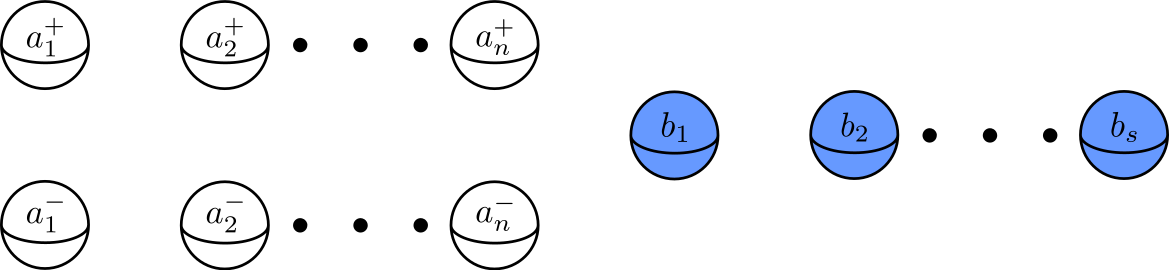
\includegraphics[width=\textwidth]{figures/spherestoglue.pdf}
  \caption{}
  \label{fig:sphereglue}
\end{figure}

\begin{theorem}[Laudenbach \cite{MR0314054}]
$\Gamma_{n,0} \cong \oout F_n$ and $\Gamma_{n,1} \cong \aaut F_n$
\end{theorem}

$\G_n$ is the graph of free splittings of $F_n$


$\mathcal S_{n,s}$ is the complex of spheres in $M_{n,s}$
whose $k$ simplices are $k+1$ disjointely essential embedded 2-spheres in $M_{n,s}$
$\mathcal S_\infty$ is the subcomplex of $\mathcal S_{n,0}$
consisting of sphere systems having at least one non-simply connected complimentary component


\begin{theorem}[Hatcher \cite{MR1314940}]
$\mathcal S_{n,0} - \mathcal S_\infty$ is homeomorphic to Culler-Vogtmann outer space
\end{theorem}

\begin{theorem}[Aramayona, Souto \cite{souto}]
\label{aramsouto}
The natural map $\oout F_n \to \aaut S_n  \cong \aaut \G_n$ is an isomorphism for $n\geq 3$.
\end{theorem}

\begin{theorem}[Pandit \cite{pandit}]
  For $n \geq 3$ we have $\Aut{\nosep} \cong \outn$.
\end{theorem}

\begin{theorem}[Putman's Lemma \cite{putman}]
  \label{putmanlemma}
  Let group $G$ with generators $H$ act on simplicial set $X$. Fix a basepoint $v \in X^{(0)}$.
  If
  \begin{enumerate}
  \item for all $v' \in X^{(0)}$ the orbit $G\cdot v$ intersects the connected component of $v'$ in $X$ and
  \item for all $h \in H^{\pm}$ there is some path from $v$ to $h\cdot v$
  \end{enumerate}
  then $X$ is connected.\\
\end{theorem}


\begin{lemma}
  An essential separating sphere of $M_{n,s}$ is uniquely determined by
  any of the following data:
  \begin{enumerate}
    \item A bipartition of any $n$ disjoint nonseparating spheres
    and the boundary spheres.
    \item A collection of $\alpha_1,\ldots, \alpha_k$
    independent loops
    and disjoint nonseparating spheres $a_1,\ldots,a_k$
    such that every $\alpha_i$ intersects a $a_j$, and a subset of the boundary spheres.
    \item
    A free splitting of each
    $\pi_1(M_{n,s},x_i)$ for a point $x_i$ on each boundary
    component, or else the conjugacy class
    of a free splitting if $s=0$.
  \end{enumerate}
  \label{lemma:sepspecify}
\end{lemma}


\section{
The Birman Exact Sequence in the Curve Complex
}

Definitions:!!!!
surface $S_{g,p}$ with marked points $P$



The purpose of this section is to sketch the surface analog of the proof we will follow for the complex of spheres.

The works of
Ivanov \cite{MR1460387},
Korkmaz \cite{MR1696431},
and
Luo \cite{MR1722024},
describe the automorphisms of complexes of curves.
Their theorem may be summarized
\begin{theorem}
  The natural map
  $$
  \mcg^\pm S_{g,p} \to  \aaut \mathcal C S_{g,p}
  $$
  is an isomorphism whenever the curve complex
  $\mathcal C S_{g,p}$
  has positive dimension $3g+p-4$ and $(g,p) \neq (1,2)$.
  \label{thm:curvecomplex}
\end{theorem}

Although their methods of proof are general and
do not require separate consideration of the closed and
punctured cases, we will demonstrate
that additional punctures of the surface
leave the isomorphism
$$
\mcg^\pm S_{g,p} \to  \aaut \mathcal C S_{g,p}
$$
intact,
if we consider the celebrated Birman exact sequence.
The Birman exact sequence
describes the
mapping class group of a punctured surface
as a fibration
over the mapping class group of the unpunctured surface,
where the fundamental group is the fiber \cite{MR0243519}.

\begin{theorem}
  Let $q\in S_{g,p}$.
  The surface inclusion $S_{g,p+1}=S_{g,p}-\{q\} \hookrightarrow S_{g,p}$
  induces the following short exact sequence
  $$
  \begin{tikzcd}
  1 \arrow[r]&
  \pi_1(S_{g,p},q) \arrow[r]&
  \mcg^{\pm}(S_{g,p+1},q)  \arrow[r]&
  \mcg^{\pm}S_{g,p} \arrow[r]&
  1
  \end{tikzcd}
  $$
  \label{thm:puncrigid}
\end{theorem}

Our goal in this subsection will be an independent proof of
the following
weaker version of Theorem \ref{thm:curvecomplex},
in preparation for the free group analog.

\begin{theorem}
  If the natural map
  $$
  \mcg^\pm S_{g,p} \to  \aaut \mathcal C S_{g,p}
  $$
  is an isomorphism, then so is
  $$
  \mcg^\pm S_{g,p+1} \to  \aaut \mathcal C S_{g,p+1}.
  $$
  \label{thm:addpunc}
\end{theorem}

The proofs of Theorems \ref{thm:addpunc} and  \ref{thm:puncrigid}



Every simplex $\Delta$ of $\mathcal C S_{g,p}$
is a collection of disjoint curves cuts up the surface $S_{g,p}$
a number of connected components.
This gives a
Bass-Serre
graph of groups \cite{MR607504} for $\pi_1 S_{g,p}$
induced by the $\Delta$ specified splitting.
The underlying simple graph
is the adjacency graph studied in
Margalit, Behrstock \cite{MR2239449}
and Shackleton \cite{MR2318453}.
Also appear as graphs associated to
pants decompositions/markings in \cite{MR579573}.

\begin{definition}
Let $\Delta \subset \mathcal C S_{g,p}$ be a simplex.
The \emph{region adjacency graph} $\mathcal G_\Delta$
of $\Delta$
is the graph whose
vertices are the connected components of
the cut surface
$$
S_{g,p} - \bigcup_{c \in \Delta} c
$$
with an edge for
every curve $c$ incident to the regions it bounds.

We will also consider the graph simplification
$\mathcal G^{simp}_{\Delta}$ obtained
from the (possibly looped, multi-edged) graph
$\mathcal G_\Delta$ by
removing any self-loops and
identifying multi-edges.
\label{def:graphadj}
\end{definition}

Automorphisms
of the curve complex act naturally on the
set of adjacency graphs by isomorphism, as we show in the
following lemma, due to Margalit and Behrstock \cite{MR2239449}.
Or Irmak?!!!!
For completeness, we argue similarly here.

\begin{lemma}
  Curve complex automorphisms preserve the
  edge incidence of region adjacency graphs.

  Let $\phi \in \aaut \mathcal C S_{g,p}$
  and let $\Delta$ be a simplex of $\mathcal C S_{g,p}$
  with adjacency graph $\mathcal G_\Delta$.
  Then $e_c,e_{c'}$ are incident edges of $\mathcal G_\Delta$
  if and only if $e_{\phi(c)},e_{\phi(c')}$
  are incident edges of $\mathcal G_{\phi(\Delta)}$.
  \label{lemma:adjgraph}
\end{lemma}

\begin{proof}
  We will argue that $\phi$ induces a map
  $\phi_\ast : E_{\mathcal G_\Delta} \to E_{\mathcal G_{\phi(\Delta)}}$
  on the set of edges
  that preserves the incidence
  and non-incidence of edges.

  Let $e_c$ be an edge of $\mathcal G_\Delta$ given by curve $c$.
  Then $\phi_\ast (e_c) = e_{\phi(c)}$  defines a bijection
  between the edges of $\mathcal G_\Delta$ and $\mathcal G_{\phi(\Delta)}$.
  We will show $e_c$ is incident to $e_{c'}$ if
  and only if there is a curve of $\mathcal C S_{g,n}$
  intersecting $c$ and $c'$, but no other curve of $\Delta$.
  Then $e_{\phi(c)}$ is incident to $e_{\phi(c')}$
  if and only if there is a curve of $\mathcal C S_{g,n}$
  intersecting $\phi(c)$ and $\phi(c')$, but no other curve of $\phi(\Delta)$.

  Suppose $e_c$ is incident to $e_{c'}$.
  Observe every region  of
  $
  S_{g,p} - \bigcup_{c \in \Delta} c
  $
  contains an embedded pair of pants $S_{0,3}$.
  So if we consider regluing regions along $c$ and $c'$,
  we obtain the
  component $R$ of $
  S_{g,p} - \bigcup_{b\neq c,c'} b
  $
  with $c,c' \subset R$.
  Then $R$ must contain an embedded $S_{0,5}$
  or a $S_{1,1}$.
  So $R$ contains a curve $c''$ intersecting $c$ and $c'$,
  and since $c'' \subset R$, it does not intersect any other curve of $\Delta$.

  Suppose $e_c$ is not incident to $e_{c'}$ in $\mathcal G_{\Delta}$.
  Then there is a multicurve $\Delta' \subset \Delta$
  which separates $c$ from $c'$ in $S_{g,p}$.
  But then every curve that intersects $c$ and $c'$ must intersect a curve of $\Delta'$.
\end{proof}

\begin{example}
  Edge incidence isn't always enough for an isomorph:
  Explain $S_1,2$, $K_3 \cong K_{1,3}$, loop-multiedge swap with 2 vertices
\end{example}


We recall the Whitney Graph Isomorphism Theorem
\cite{MR1506881}
states that the edge-incidence relation determines a simple graph,
with a single exceptional pair.

\begin{theorem}
  An edge-incidence preserving bijection between two simple, connected graphs
  is a isomorphism, provided neither is the complete graph $K_3$.

  There is an edge-incidence preserving edge bijection between the complete
  graph $K_3$ and the complete bipartite graph $K_{1,3}$.
  \label{thm:whitney}
\end{theorem}

Edge incidence can be preserve and swap a loop with a multiedge,
as in $\aaut \mathcal C S_{1,2}$,
Show example !!!!




\begin{corollary}
  Curve complex automorphisms induce isomorphisms of
  region adjacency graphs of maximal simplices, except in the case of $S_{1,2}$.

  Let $\phi \in \aaut \mathcal C S_{g,p}$ for $(g,p)\neq(1,2)$,
  and let $\Delta$ be a maximal simplex of $\mathcal C S_{g,p}$.
  Then $\mathcal G_\Delta$ and
  $\mathcal G_{\phi(\Delta)}$
  are isomorphic graphs.
  \label{cor:adjgraph}
\end{corollary}

\begin{proof}
  Any maximum simplex $\Delta$
  gives a pants decomposition!!!! of the surface $S_{g,p}$
  with $3g+p-3$ curves and $2g+p-2$ pairs of pants.
  So $\mathcal G^{simp}_\Delta$
  and
  $\mathcal G^{simp}_{\phi(\Delta)}$
  are simple, connected graphs with the same number of
  vertices and the same edge-incidence relations.
  Then by Whitney's Theorem \ref{thm:whitney},
  $\mathcal G^{simp}_\Delta$ is isomorphic to
  $\mathcal G^{simp}_{\phi(\Delta)}$.

  To see that self-loops are preserved, observe
  that as $\Delta$ cuts $S_{g,p}$ into pairs of pants,
  every vertex of $G_\Delta$ has degree at most 3.
  Then if $e_c$ is a self-loop at vertex $v_R$,
  it is incident to exactly one other edge $e_x$
  which cannot be a self-loop, so $e_x$ is uniquely represented in $\mathcal G^{simp}_\Delta$.
  If $(g,p) \neq (1,2)$, then $e_x$ is incident to another edge $e_y$.
  Then $e_\phi(x)$ is
  also uniquely represented in the isomorphic graph $\mathcal G^{simp}_\Delta$
  and has a degree 1 vertex.
  Then in $G^{simp}_\Delta$, $e_\phi(x)$
  is incident to $e_\phi(y)$, and $e_\phi(c)$ is incident to $e_\phi(x)$,
  but not $e_\phi(y)$ or any other edge, so $e_\phi(c)$   must be a loop at the vertex
  which is degree 1 in $G^{simp}_{\phi(\Delta)}$.
\end{proof}


\begin{lemma}
  For positive dimension and $(g,p)\neq(1,2)$, any automorphism of
  $ \aaut \mathcal C S_{g,p}$
  preserves the topological type of curves
  sides of separating curves.
  \label{lemma:curvetype}
\end{lemma}
\begin{proof}
  We will characterize each topological type of curve
  by a combinatorial property of a corresponding region adjacency graph,
  and apply Lemmas
  \ref{lemma:adjgraph} and \ref{cor:adjgraph}.

  \begin{enumerate}[$\cdot$]
    \item Nonseparating curves:
    Observe that a curve $c$ is nonseparating if and only if
    there is a maximal simplex $\Delta$ for which $e_c$
    is a self-loop in the region adjacency graph $\mathcal G_\Delta$.
    \item Separating curves:
    Observe that if curve $x$ separates $S_{g,p}$
    $$
    S_{g,p} = S_{g',p'} \sqcup_c S_{g-g',p-p'+2}
    $$
    then the corresponding edge $e_x$ of the
    region adjacency graph
    $\mathcal G_\Delta$
    is a cut edge.
    More specifically, if
    $$\Delta = \Delta_+ \cup \{x\} \cup \Delta_-$$
    with $\Delta_+$ and $\Delta_-$
    the curves on each side of the separating curve $c$,
    then $e_x$ separates $\mathcal G_\Delta$
    $$\mathcal G_\Delta  - \{e_x\}  = G_{\Delta_+} \sqcup G_{\Delta_-}$$
    into the components
    $G_{\Delta_+}$, with
    $3g'+p'-3$ edges and genus $g'$,
    and $G_{\Delta_-}$ with $3(g-g')+p-p'-1$ edges and genus $g-g'$.
  \end{enumerate}
  \end{proof}




\begin{remark}
For the closed surface $S_g$ the inclusion $S_{g}-\{q\} \hookrightarrow S_{g}$
has a well defined adjoint forgetful map
$$
\mathcal C S_{g,1} \to \mathcal C S_g
$$
since we do not allow peripheral curves in $\mathcal C S_{g,1}$.
However, in the case of multiple punctures $P$,
the surface $S_{g,p}$ has curves bounding twice-punctured disks,
which may become peripheral if a puncture is forgotten.
However, excluding these curves
gives a subcomplex $\mathcal C(S_{g,p},q) \subset \mathcal C S_{g,p}$
where the puncture-forgetting map is well-defined.
$$
\rho_q: \mathcal C(S_{g,p},q) \to \mathcal C S_{g,p-1}
$$

Kent, Leininger, and Schleimer \cite{MR2599078}
show that this forgetful projection has
fibers described by Bass-Serre trees of the surface fundamental group
so that there is a fibration of the form
$$
\mathcal T \to \mathcal C(S_{g,p},q) \to \mathcal C S_{g,p-1}.
$$
More rigorously,
\end{remark}

\begin{theorem}
  Let $\Delta \subset \mathcal C S_{g,p}$
  be a simplex with interior point $x \in \Delta$.
  Then the fiber $\rho^{-1}_q(x)$ is
  $\pi_1 \left ( S_{g,p}, q \right )$-equivariantly
  homeomorphic to the tree $\mathcal T_\Delta$,
  the Bass-Serre tree for the splitting of
  $\pi_1 \left ( S_{g,p}, q \right )$
  determined by the multicurve $\Delta$.
  \label{thm:kent}
\end{theorem}


Observe that $\mathcal C(S_{g,p},q)$
is not characteristic in $C S_{g,p}$,
since in general automorphisms of $C S_{g,p}$ will permute the punctures.
Let $\aaut (\mathcal C S_{g,p},q) < \aaut \mathcal C S_{g,p}$
be the subgroup of $\aaut \mathcal C S_{g,p}$
which preserves the fibration
$\mathcal C(S_{g,p},q) \to \mathcal C(S_{g,p-1})$, i.e.
$\phi \left ( \rho_q^{-1}\rho_q(x) \right ) = \rho_q^{-1}\rho_q(\phi(x))$.
These automorphisms display the structure of the Birman exact sequence.

\begin{lemma}
  This diagram commutes
  $$
  \begin{tikzcd}
  1 \arrow[r]&
  \pi_1(S_{g,p-1},q) \arrow[r] \arrow[d]&
  \mcg^{\pm}(S_{g,p},q)  \arrow{r}{f_q} \arrow[d]&
  \mcg^{\pm}S_{g,p-1} \arrow[r] \arrow[d]&
  1 \\
  1 \arrow[r]&
  \pi_1(S_{g,p-1},q) \arrow{r}{\alpha}&
  \aaut \mathcal C (S_{g,p},q)  \arrow{r}{\rho_{q}}&
  \aaut \mathcal C S_{g,p-1} \arrow{r}&
  1 \\
  \end{tikzcd}
  $$
  and has exact rows when $\rho_{q}$ is surjective.
  \label{lemma:exact}
\end{lemma}



\begin{proof}
  The map $\alpha$ is defined by the first square,
  so it certainly commutes.
  And $\alpha$
  gives a well defined injection,
  since for any nontrivial loop $\gamma$
  there is a nonseparating curve $c$
  which intersects $\gamma$ so that the push map
  $\alpha(\gamma)$ moves $c$, and $c \in \mathcal C (S_{g,p},q)$.

  The second square must commute,
  since if $[\psi] \in \mcg^\pm (S_{g,p},q)$
  is a mapping class and $c$ a curve of $S_{g,p}$,
  the homotopy class of $\psi(c)$ is the same if we first
  forget that $\psi$ fixes $q$ or if we first allow $\psi$ with
  $q$ fixed, then homotope $\psi(c)$ forgetting $q$.

  According to Theorem \ref{thm:kent},
  a fiber $\rho^{-1}_q(x)$ of the projection
  $\rho_q: \mathcal  C (S_{g,p},q) \to \mathcal C S_{g,p}$
  for $x$ in interior point of simplex $x\in \Delta$
  is homeomorphic to the Bass-Serre
  tree $\mathcal T_\Delta$.
  Then the kernel $\ker \rho_{q}$ is a
  group acting on the tree $\mathcal T_\Delta$,
  so by the
  Fundamental Theorem of Bass–Serre Theory
  (how to reference?!!!!),
  $\ker \rho_{q}$ is isomorphic to
  the fundamental group $\pi_1$ of the
  quotient graph of groups,
  but the corresponding graph of groups is
  exactly the Van Kampen splitting of $\pi_1$ induced by $\Delta$.
  Thus
  $$\ker \rho_{q} = \mbox{image } \alpha \cong \pi_1(S_{g,p},q)$$
  and the second row is exact.
\end{proof}

We will show that, though curve complex automorphisms might not
preserve the fibers of $\rho_q$ for any particular puncture $q$, they do permute the fibers
of the puncture-forgetting projections $(\rho_q)_{q \in P}$.
Korkmaz's proof of Theorem \ref{thm:curvecomplex}
utilizes a slightly more general arc complex
allowing peripheral arcs \cite{MR1696431}

\begin{definition}
  Define the arc complex complex
  $\mathcal A S_{g,p}$
  to be the complex of homotopy classes of embedded
  non-peripheral arcs in $S_{g,p}$ with endpoints in $P$,
  where an arc is peripheral if
  it is a separating loop based at a single puncture,
  and one of its sides is a punctured monogon of $S_{g,p}$.
  Two arcs are adjacent in
  $\mathcal A S_{g,p}$ if their homotopy classes
  have disjoint representatives and share no punctures as endpoints.
\end{definition}

\begin{remark}
  The arc complex has as vertices
  both arcs with two distinct
  endpoints and loops based at a single puncture.
  Since loops that are disjoint are always
  based at distinct punctures,
  there is an obvious way to color (in the graph-theoretic sense)
  the loop-vertices of
  $\mathcal A S_{g,p}$:
  assign a color to each puncture and all the loops based at that puncture.
  The arcs with distinct endpoints
  require two colors, however.
  We make a slight generalization of
  $k$-colorings to allow a privileged set of vertices that
  which require two colors.
\end{remark}

\begin{definition}
  A $k,\eta$-painting of a graph $G=(V,E)$
  is an assignment
  to each vertex $v$ of a number of colors $\eta(v)$
  and
  a choice $f(v) \subset \{0,\ldots,k-1\}$ of $\eta(v)$
  colors
  such that two adjacent vertices have no common colors.
  I.e. functions $\eta: V \to \Z_+$ and  $f: V \to 2^{\{0,\ldots,k-1\}}$
  so that $|f(v)| = \eta(v)$
  and
  $$f(v) \cap f(u) = \varnothing$$
  if $v$ is adjacent to $u$ in $G$.
  Call $G$ $k$-paintable if it admits a $k,\eta$-painting.
\end{definition}


MOVE THIS TO INTROMATERIAL?
Margalit in \cite{MR2040283} discusses the
trinion pants complex.
Pants decompositions of $S_{g,p}$ are maximal simplices of
$\mathcal C S_{g,p}$,
with two such pants decompositions giving sharing
an edge in the pants complex if they differ
by a single pair of minimally intersecting curves.
Hatcher and Thurston
demonstrated the
pants complex (which they call \emph{markings}) of a surface
is connected and simply connected
in \cite{MR579573}.
We recall their result as the following helpful lemma.

\begin{lemma}
  Let $\Delta,\Delta'$ be maximal $k$-simplicies of $\mathcal C S_{g,p}$.
  Then there is a sequence $\Delta = \Delta_0, \Delta_1, \ldots, \Delta_n=\Delta'$
  of maximal simplices such that
  $\Delta_i \cap \Delta_{i+1}$ is a $k-1$ simplex
  and the curves $c_i \in \Delta_i - \Delta_{i+1}$
  and $c'_i \in \Delta_{i+1} - \Delta_i$
  are contained in a single component $R$ of
  $S_{g,p} - \bigcup_{x \in \Delta_i \cap \Delta_{i+1}} x$.
  Further,
  $c_i,c'_i$ can be chosen to intersect once if $R \cong S_{1,1}$
  and twice if $R \cong S_{0,4}$.
  \label{lemma:pantspath}
\end{lemma}

\begin{lemma}
  The arc complex is uniquely paintable.

  Let $3g+p\geq6$.
  The arc complex $\mathcal A S_{g,p}$,
  it admits a
  unique
  $p$-painting,
  up to permutation of the colors.
  \label{lemma:paint}
\end{lemma}

\begin{proof}
  We will argue with a modification of the Putman trick \ref{putmanlemma}.
  Observe that (since we exclude peripheral arcs)
  every maximal simplex of $\mathcal A S_{g,p}$
  has an arc with an end at every puncture.
  Observe that if $p \leq 2$ the result is trivial,
  so we assume $p \geq 3$.
  Let $f$ be any $p$-coloring of the
  arc complex $\mathcal A S_{g,p}$.

  \begin{figure}
    \includegraphics[width=.6\textwidth]{figures/pcolorgenus.pdf}
    \caption{A base collection of parallel nonseparating loops.}
    \label{fig:pcolorg}
  \end{figure}

  We first fix a collection $X$ of curves.
  If $g\geq1$, then $S_{g,p}$ has a nonseparating curve,
  and we let $X$ contain $p$ parallel nonseparating loops based at the punctures
  as in Figure \ref{fig:pcolorg}.


  If $g=0$ we take as $X=\{x_i\}_{i=1}^p$ to be as in Figure \ref{fig:pcolors}
  with $p-4$ parallel loops based at $p_2,\ldots,p_{p-2}$
  and 4 additional curves $x_1,x_2,x_{p-1},x_p$
  so that $x_1$, $x_2$ and $x_3$ pairwise intersect twice
  and are disjoint from all other curves of $X$,
  and similarly $x_p,x_{p-1},x_{p-2}$ pairwise intersect twice
  and are disjoint from all other curves of $X$.
  We will argue that each loop of $X$ must be colored differently.
  Observe that there is an arc
  $\alpha_{12}$
  from $p_1$ to $p_2$
  which is disjoint from all loops of $X$ except $x_1$ and $x_2$.
  Similarly
  there is  $\alpha_{p-1,p}$
  disjoint from all loops of $X$ except $x_p$ and $x_{p-1}$.
  So the collection $\alpha_{12},x_3,\ldots,x_{p-2},\alpha_{p-1,p}$
  require all $p$-colors to paint,
  and it must be that $f(x_1)\cup f(x_2) = f(\alpha_{12})$
  and $f(x_{p-1})\cup f(x_p) = f(\alpha_{p,p-1})$.
  So $X$ requires $p$-colors to paint.

  \begin{figure}
    \includegraphics[width=.6\textwidth]{figures/pcolorspher.pdf}
    \caption{A base collection of mostly parallel loops in the punctured sphere.}
    \label{fig:pcolors}
  \end{figure}


  We may then assume, possibly after relabeling the colors,
  that $f$ colors the arcs of $X$ by their punctures.
  We will show that the painting on $X$ forces
  the painting on all of $\mathcal A S_{g,p}$.
  Our technique will be to contruct paths with the group action
  of $\mcg S_{g,p}$ on $\mathcal A S_{g,p}$
  and show that $f$ is determined along these paths.
  Let $\alpha_{i,i+1}$ be an arc which is disjoint from
  all loops of $X$ except $x_i$ and $x_{i+1}$
  and contained in the annulus they bound if they are disjoint.
  Take as a generating set of $\mcg S_{g,p}$
  the Dehn half-twists along the arcs $\alpha_{i,i+1}$
  and the usual Humphrey's generators
  of Dehn twists about nonseparating curves
  which are disjoint from $X$, except for one curve $z$
  which intersects each loop of $X$ exactly once.

  We now claim that for $h \in H$ the
  painting $f$ is determined on the loops $h\cdot X$
  by the painting on $X$.
  We must consider several cases
  depending on whether $h$ is a twist or half-twist,
  and how $\alpha_{i,i+1}$ intersects $X$.
  These cases are considered in Figures \ref{fig:pcolor1}-\ref{fig:pcolor4}.
    \begin{figure}[h!]
      \includegraphics[width=.7\textwidth]{figures/pcolorsequence1.pdf}
      \caption{Case 1: The half-twist $h$ is about an arc $\alpha$
      in an annulus between $x_i$ and $x_{i+1}$ and disjoint from the other loops of $X$,
      as in the top left.
      The lower right shows $h(x_1)$, $h(x_2)$, and $h(x_3)=x_3$.
      Then if $f(x_i)=p_i$ the sequence of curve replacements shows
      that $f(h(x_i))=p_i$.
      }
      \label{fig:pcolor1}
    \end{figure}
    \begin{figure}[h!]
      \includegraphics[width=.5\textwidth]{figures/pcolorsequence2.pdf}
      \caption{Case 2: The half-twist $h$ is about an arc $\alpha$
      $x_i$ and $x_{i+1}$ and disjoint from the other loops of $X$,
      where $x_i$ and $x_{i+1}$ intersect twice.
      We may assume the configuration on the left and note that
      $h(x_2)=x_3$, so that $f(h(x_3))$ must be $p_2$.}
      \label{fig:pcolor2}
    \end{figure}
    \begin{figure}[h!]
      \includegraphics[width=.8\textwidth]{figures/pcolorsequence3.pdf}
      \caption{Case 3: The half-twist $h$ is about arc $\alpha$
      between disjoint curves $x_i$ and $x_{i+1}$,
      and $\alpha$ intersects other curves of $X$.
      We may assume the configuration on the top left.
      Then the image of $h$ is shown in the bottom right.
      Note that by Case 1, $f(h(x_3))=p_3$ and $f(h(x_4))=p_4$
      so that we need only determine $f(h(x_1))$ and $f(h(x_2))$.
      }
      \label{fig:pcolor3}
    \end{figure}
    \begin{figure}[h!]
      \includegraphics[width=1\textwidth]{figures/pcolorsequence4.pdf}
      \caption{Case 4: The Dehn twist $h=T_z$ about a nonseparating curve
      which links with the loops of $X$.
      We may assume the configuration of $X$ and $z$ as in the top left.
      The image $T_z(X)$ is shown in the bottom right.
      In the top row: Replace $x_1$ and $x_2$ with $\alpha_{1,2}$
      so that $f(\alpha_{12})=\{p_1,p_2\}$.
      Then iteratively replace $x_k$ with the loop $y_k$ separating
      $\alpha_{1,2},y_3, \ldots, y_{k-1}$ from the other punctures,
      so that $f(y_k)=p_k$ for $k=3,\ldots,p$.
      Then replace $y_k$ with $h(x_k)$ so that $f(T_z(x_k))=p_k$
      for $k=p, \ldots, 3$.
      A similar process reversing the order of the punctures
      as in the bottom row shows $f(T_z(x_k))=p_k$ for $k=1,\ldots,p-2$.
      }
      \label{fig:pcolor4}
    \end{figure}

  Observe that if $g \in \mcg S_{g,p}$
  we can write $g= h_n \cdots h_1$ with $h_i \in H$.
  And if the loops of $h_k \cdots h_1 \cdot X$ are painted by their punctures,
  then so are the loops of $h_{k+1} \cdots h_1 \cdot X$ by the above argument.

  Observe in the case of $g=0$ every curve is in $\mcg S_{g,p} \cdot X$.
  If $g \geq 1$ then $\mcg S_{g,p} \cdot X$ includes all nonseparating loops,
  and any separating loop $x$ is disjoint from $p-1$ mutually disjoint loops $x_1,\ldots, x_{p-1}$
  so that
  the color $f(x)$ is determined by
  the colors
  $f(x_i)$
  and so $f(x)$ must be colored by its puncture.
\end{proof}


\begin{lemma}
  Curve complex automorphisms induce
  arc complex $\mathcal A S_{g,p}$
   automorphisms.
  \label{lemma:annulus}
\end{lemma}

\begin{proof}
  By Lemma \ref{lemma:curvetype}
  automorphisms of $\mathcal S_{g,p}$
  preserve the class of two curves.
  Observe that curves $c,c'$ of $S_{g,p}$
  bound a punctured annulus if and only if there
  is a maximal simplex $\Delta \subset \mathcal C S_{g,p}$
  containing $c,c'$
  so that in the region adjacency graph $\mathcal G_\Delta$,
  the edges $e_c$ and $e_{c'}$ are incident
  at a degree 2 vertex $v_a$.
  Then applying Lemma \ref{cor:adjgraph}
  $\phi(c)$ and $\phi(c')$ must cobound a punctured annulus.

  Let $\phi \in \aaut \mathcal C S_{g,p}$
  and let $a$ be an punctured annulus $\mathcal A S_{g,p}$
  with bounding curves $c,c'$.
  If $(g,p) \neq (1,2)$ then $c,c'$ uniquely specify the annulus.
  Then $\phi(c),\phi(c')$ specify cobound a punctured annulus $\phi_\ast(a)$.

  Finally $a,a'$ are disjoint arcs if and only if
  there is a maximal simplex $\Delta \subset \mathcal C S_{g,p}$
  such that the bounding curves of regular neighborhoods of
  $a$ and $a'$
  are in $\Delta$.
  Then $a$ and $a'$ are represented by distinct
  vertices $v_a$ and $v_{a'}$ of $\mathcal G_\Delta$.
  So $a$ and $a'$ are disjoint if and only if
  $\phi_\ast (a)$ and $\phi_\ast (a')$ are disjoint.

  Thus $\phi_\ast : \mathcal A S_{g,p} \to \mathcal A S_{g,p}$
  is an isomorphism.
\end{proof}





\begin{lemma}
  Curve complex automorphism permute puncture-projection fibers.

  Let $\phi \in \aaut \mathcal C S_{g,p}$ for $3g+p \geq 6$.
  Then if $x,y$ are curves of $S_{g,p}$ with
  $\rho_q(x)=\rho_q(y)$,
  then there is a puncture $q' \in P$ such that
  $\rho_{q'}(\phi(x))=\rho_{q'}(\phi(y))$.
  \label{lemma:fibers}
\end{lemma}

\begin{proof}
  Consider the structure of $\rho^{-1}_q(\rho_q(x))$.
  We have it is a subtree of $\mathcal C S_{g,p}$
  with $x,x' \in \rho^{-1}_q(\rho_q(x))$
  adjacent if and only if they bound an annulus punctured by $q$.
  Then we have a path $x=x_0 \to \ldots \to x_n =y$
  such that $x_i,x_{i+1}$ bound an annulus punctured by $q$.
  Using \label{lemma:annulus}
  we have $\phi(x_i),\phi(x_{i+1})$ bound an annulus
  punctured by some $q_i$.
  Then since $x_i,x_{i+1},x_{i+2}$ bound
  annuli  punctured by $q$,
  which  are the regular neighborhoods of
  loops $a_i,a_{i+1} \in \mathcal A S_{g,p}$ based at $q$.
  Then
  $\phi(x_i),\phi(x_{i+1}), \phi(x_{i+2})$
  bound annuli which are the regular neighborhoods
  of loops $\phi_\ast(a_i), \phi_\ast(a_{i+1})$.
  By Lemma \ref{lemma:paint}
  $\phi_\ast(a_i)$ and $\phi_\ast(a_{i+1})$
  are based at a common point $q'$.
\end{proof}


\begin{proof}[Proof of Theorem \ref{thm:addpunc}]
  Assume that the natural map
  $$
  \begin{tikzcd}
  \mcg^{\pm}S_{g,p-1} \arrow{r}{\gamma}& \aaut \mathcal C S_{g,p-1}
  \end{tikzcd}
  $$
  is an isomorphism.
  Then by Lemma
  \ref{lemma:exact}
  the following diagram commutes
  $$
  \begin{tikzcd}
  1 \arrow[r]&
  \pi_1(S_{g,p-1},q) \arrow[r] \arrow{d}{\alpha}&
  \mcg^{\pm}(S_{g,p},q)  \arrow{r}{f_q} \arrow{d}{\beta}&
  \mcg^{\pm}S_{g,p-1} \arrow[r] \arrow{d}{\gamma}&
  1 \\
  1 \arrow[r]&
  \pi_1(S_{g,p-1},q) \arrow{r}&
  \aaut \mathcal C (S_{g,p},q)  \arrow{r}{\rho_q}&
  \aaut \mathcal C S_{g,p-1} \arrow{r}&
  1. \\
  \end{tikzcd}
  $$
  and since $\gamma f_q = \rho_q \beta$ is a surjection we have
  that $\rho_q$ is a surjection and the rows are exact.
  By the Five Lemma $\beta$ is an isomorphism.

  Let $\phi \in \aaut \mathcal C S_{g,p}$.
  We have that by Lemma
  \ref{lemma:fibers} that
  $\phi$ permutes the fibers $\{\rho^{-1}_q\}$,
  so there is $\psi \in \mcg^{\pm}S_{g,p}$
  so that $\psi_\ast \in \aaut \mathcal C S_{g,p}$
  is such that $\psi_\ast \phi$ maintains the fibers
  $\rho^{-1}_q$.
  So $\psi_\ast \phi \in \aaut \mathcal C(S_{g,p},q)$.
  But then there is $\psi' \in \mcg^{\pm}S_{g,p}$
  so that $\psi_\ast \phi = \psi'_\ast$.
  But then $\phi = \left ( \psi^{-1}\psi' \right)_\ast$
  is also induced by a mapping class we have the natural map
  $$
  \begin{tikzcd}
  \mcg^{\pm}S_{g,p} \arrow{r} & \aaut \mathcal C S_{g,p}
  \end{tikzcd}
  $$
  is an isomorphism.
\end{proof}

\section{All Mapping Class Group Extensions are Products}

See the primer \cite{primer}
\begin{theorem}
  The center of $\mcg S_{g,p}$ is trivial, unless
  $$(g,p) \in \left\{ (0,2), (1,0),(1,1),(1,2),(2,0) \right\}$$
  and in all these cases $Z\left ( \mcg S_{g,p} \right ) \cong \Z/2$.
  \label{nocenter}
\end{theorem}

This is also obviously true for $\mcg^{\pm}$,
but perhaps I must argue it.
Mirror reflection doesn't commute with Dehn twisting.

McCarthy \cite{MR830038},
Ivanov \cite{MR1460387},
Korkmaz \cite{MR1696431}
\begin{theorem}
Let $(g,p)$ have $g\geq 2$ and $g+p \geq 3$,
or $g=1$ and $p\geq 3$, or $g=0$ and $p \geq 5$.
Let $G$ and $G'$ be finite index subgroups of $\mcg^\pm S_{g,p}$.
Then any isomorphism $G\to G'$ is induced by an inner automorphism of $\mcg^\pm S_{g,p}$.
\label{outmod}
\end{theorem}

In general the isomorphism class of a fibration of groups
$$
\begin{tikzcd}
  1 \arrow[r] &
  A \arrow[r]&
  E \arrow[r]&
  B \arrow[r]&
  1
\end{tikzcd}
$$
is classified by an $\oout G$ and
the cohomology $H^\ast (B;Z(A))$
see e.g. Brown \cite{MR1324339}.
But mapping class groups are centerless and out-less!

\begin{theorem}
  A centerless, out-less group always fibers trivially.

  Suppose that
  $$
  \begin{tikzcd}
    1 \arrow[r] &
    A \arrow[hook,r]&
    E \arrow[two heads]{r}{\pi}&
    B \arrow[r]&
    1
  \end{tikzcd}
  $$
  is a short exact sequence of groups.
  If $A$ has trivial center and outer automorphism group,
  then $E \cong A \times B$.
\end{theorem}

\begin{proof}
Let $B = \langle S | R \rangle$
be a presentation for $B$.
For each $s\in S$ choose $e_s \in E$
so that $\pi(e_s) =s$.
Note that $A = \ker \pi$ is normal in $E$.
So the conjugation
$x \mapsto e_s x e_s^{-1}$
restricts to an automorphism of $A$.
By hypothesis $\aaut A = \mbox{Inn } A$,
so there must be $a_s \in A$ such that
$e_sx e_s^{-1} =a_s x a_s^{-1}$ for all $x \in A$.
Since
$$
\pi (e_s) = \pi (e_sa^{-1}_s) = s
$$
we may replace $e_s$ with $e_sa^{-1}_s$
so that $e_sxe^{-1}_s = x$ for all $x \in A$.
So $\langle e_s \rangle_{s \in S}$ commutes with $A$ in $E$.
But then if $\prod_i s_i \in R$ is a relation of $B$,
we have $\prod_i e_{s_i}  \in A$ by the exact sequence,
so $\prod_i e_{s_i} \in Z(A)$ is in the center of $A$.
But by hypothesis $Z(A) \cong 1$, so $\prod_i e_{s_i}=1$ in $E$.
So $s \mapsto e_s$ is a homomorphism $B \to E$ which splits the exact sequence,
and we have $E \cong A \times B$.
\end{proof}

\begin{corollary} The mapping class group has only trivial extensions.
  (Or gives only trivial fibers?)

  Let $(g,p)$ have $g\geq 2$ and $g+p \geq 3$,
  or $g=1$ and $p\geq 3$, or $g=0$ and $p \geq 5$.
  Suppose that
  $$
  \begin{tikzcd}
    1 \arrow[r] &
    \mcg^{\pm} S_{g,p} \arrow[hook,r]&
    E \arrow[two heads]{r}&
    B \arrow[r]&
    1
  \end{tikzcd}
  $$
  is an exact sequence of groups.
  Then $E \cong B \times \mcg^{\pm} S_{g,p}$.
\end{corollary}

\section{The Punctured Sphere Complex}


$\Gamma'_{n,p} =\pi_0 Diff(M_{n,p})$ i.e. don't fix boundary components.
There is an exact sequence
$$
\begin{tikzcd}
1 \arrow[r]&
\Gamma_{n,p} \arrow[r]&
\Gamma'_{n,p}  \arrow[r]&
\mbox{Sym}(p) \arrow[r]&
1
\end{tikzcd}
$$

We can describe a generating set for $\Gamma'_{n,p}$.
By capping every boundary component of
$M_{n,p}$ with a copy of $M_{1,1}$
we can include
 $\Gamma'_{n,p} \hookrightarrow \oout F_{n+p}$
and consider diffeomorphisms of $M_{n+p,0}$
which preserve (setwise with orietation) the set of separating spheres
where we glued the capping $M_{1,1}$ and the nonseparating spheres contained inside.
Consider a free basis $F_{n+p}$
given by $a_1,\ldots, a_n, b_1, \ldots, b_p$.
Then $\Gamma_{n,p}$ is generated by
\begin{enumerate}
  \item permutations of $\{a_1, \ldots, a_n\}$
  \item inversion: $a_1 \mapsto a_1^{-1}$
  \item transvection: $a_1 \mapsto a_1a_2$
  \item $a$-conjugation of $b$: $b_i \mapsto a_1b_ia_1^{-1}$
\end{enumerate}
and $\Gamma'_{n,s}$ by the addition of permutations of $\{b_1, \ldots, b_p\}$.

The usual transvection  $a_1 \mapsto a_1a_2$ corresponds to cutting the nonseparating sphere
representing $a_1$, then pushing $a_1^-$ through $a_2^-$ before regluing
$a_1^+$ and $a_1^-$.
The map $b_1 \mapsto a_1b_1a_1^{-1}$ corresponds to pushing the
bounding sphere through $a_1^+$.





This belongs in an intro about OUT and relative OUT
Out is like the projectivization of Aut, $b$ is like the point at infinty



The main theorem of this section is the following

\begin{theorem}
The natural map
$\oout (F_n,F_s) \to \aaut \mathcal S_{n,s}$ is an isomorphism for $n\geq 3$ and $s \geq 0$.
\end{theorem}

The proof is directly analogous to our proof of Theorem
\ref{thm:addpunc}.
Induct on the number of punctures.
A base, unpunctured case is considered by the Theorem of Aramayona and Souto \cite{souto}.
We will show that automorphisms of the punctured sphere complex
respect the fibration induced by forgetting punctures,
so that adding additional punctures expands the automorphism group
of the complex of spheres according to a Birmann exact sequence.

\begin{theorem}
  If the natural map
  $$
  \mcg^\pm S_{g,p} \to  \aaut \mathcal C S_{g,p}
  $$
  is an isomorphism, then so is
  $$
  \mcg^\pm S_{g,p+1} \to  \aaut \mathcal C S_{g,p+1}.
  $$
  \label{thm:outpunc}
\end{theorem}

\begin{definition}
  As in Definition \ref{def:graphadj} for surfaces,
  let $\Delta \subset \mathcal S_{g,p}$ be a simplex.
  The \emph{region adjacency graph}
  $\mathcal G_\Delta$
  of $\Delta$
  is the graph whose vertices are the connected components
  of the cut manifold
  $$
  M_{n,p} - \bigcup_{x \in \Delta} x
  $$
  with an edge $e_x$ for every sphere $x$ and with
  the edge $e_x$ incident to the connected components it bounds.

  We will also consider the graph simplification
  $\mathcal G^{simp}_\Delta$.
\end{definition}

\begin{lemma}
  Sphere complex automorphisms preserve edge incidence of region adjacency graphs.

  Let $\phi \in \aaut \mathcal S_{n,p}$ and let $\Delta$ be a simplex of $\mathcal S_{n,p}$ with adjacency graph $\mathcal G_\Delta$.
  Then $e_x, e_{x'}$ are incident edges of $\mathcal G_\Delta$
  if and only if $e_{\phi(x)}, e_{\phi(x')}$ are incident
  edges of $\mathcal G_\phi(\Delta)$.
  \label{lemma:outlinegraph}
\end{lemma}

\begin{proof}
  We will argue that the induced bijection  $\phi_\ast$
  between the edges of $\mathcal G_\Delta$ and the edges of $\mathcal G_{\phi(\Delta)}$ preserves incidence.

  Let $x,x' \in \Delta$ be distinct spheres of $M_{n,p}$.
  Suppose that the associated edges $e_x$ and $e_x'$
  of $\mathcal G_\Delta$.
  It suffices to show that $e_x$ and $e_{x'}$ are incident if and only if there is a third $y \in \Delta$ with $y$
  intersecting $x$ and $x'$ but no other sphere of $\Delta$.
  In that case $e_{\phi(x)}$ and $e_{\phi(x')}$ are incident if and only if there is no third $\phi(y) \in \phi(\Delta)$ with $\phi(y)$
  intersecting $\phi(x)$ and $\phi(x')$ but no other sphere of $\phi(\Delta)$.
  So $\phi$ induces an incidence-preserving edge bijection between $\mathcal G_\Delta$ and $\mathcal G_{\phi(\Delta)}$.

  Suppose that $e_x$ and $e_{x'}$ are incident.
  Then there is a region $R$ of $M_{n,p}-\bigcup_{z \neq x,x'}z$
  containing $x$ and $x'$, and since every region of
  $M_{n,p}-\bigcup_{z \in \Delta}z$ contains at least an $M_{0,3}$,
  it must be that $R$ contains a $M_{1,2}$ or $M_{0,5}$.

  If $R$ contains a $M_{1,2}$ the subcomplex of spheres in $R$ contains a copy of $\mathcal S_{1,2}$ and so must have infinite diameter. So there must be a sphere $y$ in $R$ that intersects both $x$ and $x'$. Since $y$ is in $R$, it intersects no other sphere of $\Delta$.

  If $R$ is simply connected then it must have a copy of $M_{0,5}$
  and $x$ and $x'$ are essential and separating in $R$.
  Then there are two boundary spheres $y',y''$ of $R$ with a path $\alpha$ between them that passes through both $x$ and $x'$. Let $y$ be the boundary of a regular neighborhood of $\alpha \cup y' \cup y''$ in $R$. Then $y$ intersects both $x$ and $x'$, but since $y$ is in $R$, $y$ does not intersect any other sphere of $\Delta$.

  Suppose that $e_x$ and $e_{x'}$ are not incident.
  Then there is a collection of spheres $\Delta' \subset \Delta$
  that separate $x$ from $x'$ in $M_{n,p}$.
  So any sphere intersecting $x$ and $x'$ must also intersect a sphere of $\Delta$.
\end{proof}



\begin{corollary}
  Sphere complex automorphisms preserve the adjacency graphs of maximal simplices.

  Let $3n+p\geq 6$.
  Let $\phi \in \aaut \mathcal S_{n,p}$ and let $\Delta$ be a maximal simplex. Then $\mathcal G_\Delta$ and $\mathcal G_{\phi(\Delta)}$
  \label{lemma:outadjgraph}
\end{corollary}

\begin{proof}
  Any maximum simplex $\Delta$ contains
  $3n+p-3$ spheres and cuts $M_{n,p}$ $2n+p-2$ copies of  $M_{0,3}$.
  So $\mathcal G^{simp}_\Delta$ and $\mathcal G^{simp}_{\phi(\Delta)}$
  are simple, connected graphs with the same number of vertices and the same edge incidence relations.
  So by Whitney's Theorem  \ref{thm:whitney},
  $\mathcal G^{simp}_\Delta$ and $\mathcal G^{simp}_{\phi(\Delta)}$
  are isomorphic.

  To see that self-loops are preserved,
  observe that as $\Delta$ cuts $M_{n,p}$ into copies of $M_{0,3}$,
  every vertex of $\mathcal G_\Delta$ has degree at most 3.
  Then if $e_x$ is a self-loop at vertex $v_R$ it is incident to exactly one other edge $e_{x'}$ which cannot be a self-loop or have a parallel edge since $v_R$ is degree 3.
  So $e_{\phi(x')}$ has a degree one vertex in $\mathcal G^{simp}_{\phi(\Delta)}$.
  Since $3n+p-3\geq 3$ we have $\mathcal G_{\phi(\Delta)}$
  has at least 3 edges.
  So if both vertices of $e_{\phi(x')}$
  are degree one in $\mathcal G^{simp}_{\phi(Delta)}$, then $\mathcal G_{\phi(Delta)}$
  has two vertices with a self loop at each.
  So $e_{\phi(x)}$ is a self loop.
  If $e_{\phi(x')}$ has only one degree one vertex in $\mathcal G^{simp}_{\phi(Delta)}$, then $e_{\phi(x)}$ is only incident to $e_{\phi(x')}$. So $e_{\phi(x)}$ must be a self loop in  $\mathcal G_{\phi(\Delta)}$.

  If $\phi$ preserves both the graph simplification and the self loops of $\mathcal G_\Delta$, it must be that $\phi$ also preserves the multi-edges, and so $\phi$ induces a graph isomorphism.
\end{proof}

\begin{lemma}
  Sphere complex automorphisms preserve the topological type of spheres, and the sides of the spheres.

  Let $3n+p\geq 6$.
  Let $\phi \in \aaut \mathcal S_{n,p}$.
  Let $x$ be a sphere of $M_{n,p}$.
  Then $x$ and $\phi(x)$ have the same topological type.
  Further if $x$ is separating and $y,y'$ are spheres in the same connected component of $M_{n,p}-x$, then $\phi(x)$ is separating and $\phi(y),\phi(y')$ are
  in the same connected component of $M_{n,p}-\phi(x)$.
  \label{lemma:outspheretype}
\end{lemma}

\begin{proof}
    By Lemma \ref{lemma:outadjgraph}
    it suffices to characterise the topological type and sides of a sphere in terms of the region adjacency graph of a maximal simplex.
    \begin{enumerate}[$\cdot$]
    \item Nonseparating spheres:
    Observe that $x$ is a nonseparating sphere if and only if there is a maximal simplex $\Delta$ in which the corresponding edge $e_x$ is a self-loop in the region adjacency graph $\mathcal G_\Delta$.
    \item Separating spheres:
    Observe that if $x$ separates $M_{n,p}$
    $$
    M_{n,p} = M_{n',p'} \sqcup_x M_{n-n',p-p'+2}
    $$
    if and only if the corresponding edge $e_x$ of the region
    adjacency graph $\mathcal G_\Delta$ is a cut edge.
    More specifically, if
    $$
    \Delta=\Delta_+ \cup \{x\} \cup \Delta_-
    $$
     with $\Delta_+$ and $\Delta_-$ the spheres on each side of $x$,
     then $e_x$ separates $\mathcal G_\Delta$
     $$
     \mathcal G_\Delta - e_x = \mathcal G_{\Delta_+} \sqcup \mathcal G_{\Delta_-}
     $$
     into the components $\mathcal G_{\Delta_+}$
     with $3n'+p'-3$ edges and rank $n'$,
     and $\mathcal G_{\Delta_-}$ with
     with $3(n-n')+p-p'-1$ edges and rank $n-n'$.
  \end{enumerate}
\end{proof}

\begin{remark}
  Consider the inclusion which ignores the puncture $q$
  $$i_q: M_{n,p} \hookrightarrow M_{n,p-1}.$$
  Then for the homotopy class $[x]$ of a sphere
  in $M_{n,p}$ we have the class $[i_q(x)]$ in $M_{n,p-1}$
  by forgetting the puncture $q$.
  Separating spheres of $M_{n,p}$ bounding a copy of $S^3$ containing only $q$ and one other puncture
  will become non-essential in this inclusion,
  but other homotopy classes of spheres have well defined
  essential representatives up to homotopy forgetting $q$.

  Let $\mathcal S_{n,p}^{(q)} \subset \mathcal S_{n,p}$
  be the subcomplex for which the puncture forgetful map
  $\rho_q: [x] \mapsto [i_q(x)]$ is well defined.
  So we have a surjective projection map
  $$
  \rho_q: \mathcal S_{n,p}^{(q)} \to \mathcal S_{n,p-1}.
  $$

As in the case for surfaces, the fibers of this map are Bass-Serre trees.
% Let $\Delta$ be a simplex in $\mathcal S_{n,p-1}$.
% Let $\Delta'$ be a simplex of $\mathcal S_{n,p}$ such that $\rho_q(\Delta')=\Delta$.
Let $x$ be a sphere of $\mathcal S_{n,p-1}$.
Homotope $x$ in $M_{n,p-1}$ so that it is pointed at $q$.
Then the two boundary  spheres of a regular neighborhood of $x$ in $M_{n,p-1}$ gives a well edge of $\rho^{-1}_q(x) \subset \mathcal S_{n,p}$.
Let $\Gamma$ be the corresponding
be the graph of groups given by the splitting of $F_n=\pi_1(M_{n,p-1},q)$.
So the vertices of $\Gamma$ are the components of
$M_{n,p-1}-x$ with vertex groups given by the $\pi_1$ of the component,
and an edge with trivial edge group between two components if $x$ is separating, or a self-loop if $x$ is nonseparating.
Then there is a an isomorphism between
$\rho_q^{-1}(x)$ and the Bass-Serre tree $\tilde \Gamma$
given by associating every edge $xx'$ of $\rho_q^{-1}(x)$
with the edge of $\Gamma$ given by $uv$
if
$$
\mbox{stab}_{\pi_1(M_{n,p-1},q)}(u)
\ast
\mbox{stab}_{\pi_1(M_{n,p-1},q)}(v)
$$
is the splitting specified
by the pointed sphere at $q$ whose regular neighborhood in $M_{n,p}$ has boundary spheres
$x$ and $x'$.
\end{remark}

% \begin{lemma}
%   The fiber of the puncture forgetful map is isomorphic to the Basse Serre tree of the splitting
%   \label{lemma:outfibershape}
% \end{lemma}

\begin{definition}
  Let $\aaut(\mathcal S_{n,p},q) < \aaut \mathcal S_{n,p}$
  be the subgroup which preserves the fibration of
  the forgetful map $\rho_p$.
  That is $\phi \in \aaut(\mathcal S_{n,p},q)$
  if
  $$
  \phi \left( \rho_p^{-1}\rho_p(x) \right)
  =
  \rho_p^{-1}\rho_p( \phi(x))
  $$
  $\pi_1(M_{n,p-1},q)$
\end{definition}

\begin{lemma}
  This diagram commutes
  $$
  \begin{tikzcd}
  1 \arrow[r]&
  \pi_1(M_{n,p-1},q) \arrow[r] \arrow[d]&
  \Gamma_{n,p}^{(q)}  \arrow{r}{f_q} \arrow[d]&
  \Gamma_{n,p-1} \arrow[r] \arrow[d]&
  1 \\
  1 \arrow[r]&
  \pi_1(M_{n,p-1},q) \arrow{r}{\alpha}&
  \aaut (\mathcal S_{n,p}, q)  \arrow{r}{\rho_{q}}&
  \aaut \mathcal S_{n,p-1} \arrow{r}&
  1 \\
  \end{tikzcd}
  $$
  and has exact rows when $\rho_{q}$ is surjective.
  \label{lemma:exact}
\end{lemma}

\begin{proof}
  The map $\alpha$ is defined by the first square, so it commutes.
  The map $\alpha$ is injective, since
  for any loop $\gamma$ based at $q$,
  there is a nonseparating sphere $x$ intersecting $\gamma$
  so that the push map $\alpha(\gamma)$ acts non-trivially on $x$ and so cannot be the identity on $\mathcal S_{n,p}^{(q)}$.

  The second square must commute,
  since if $[\psi] \in \Gamma_{n,p}^{(q)}$
  is a mapping class of $M_{n,p}$ and $x$ a sphere of $M_{n,p}$,
  the homotopy class of $\psi(x)$ is the same if we first
  forget that $\psi$ fixes $q$ or if we first allow $\psi$ with
  $q$ fixed, then homotope $\psi(x)$ forgetting $q$.

  A fiber $\rho^{-1}_q(x)$ of the forgetful map
  $\rho_q: \mathcal  S_{n,p}^{(q)} \to \mathcal  S_{n,p-1}$
  is isomorphic to the Bass-Serre tree associated to the splitting.
  Then the kernel $\ker \rho_{q}$ is a
  group acting on the tree $\mathcal T_\Delta$,
  so by the
  Fundamental Theorem of Bass–Serre Theory
  \ref{thm:bassserre},
  $\ker \rho_{q}$ is isomorphic to
  the fundamental group $\pi_1$ of the
  quotient graph of groups,
  but the corresponding graph of groups is
  exactly the Van Kampen splitting of $\pi_1$ induced by $x$.
  Thus
  $$\ker \rho_{q} = \mbox{image } \alpha \cong \pi_1(S_{g,p},q)$$
  and the second row is exact.
\end{proof}

\begin{remark}
  The edges of the fibers of the forgetful map
  are between two spheres which cobound a
  $S^2 \times I$
  punctured by $q$.
  Such spheres are specified by the boundaries of regular neighborhoods of pointed spheres of $M_{n,p}$,
  so we consider the associated complex.
\end{remark}

\begin{definition}
  Let $\mathcal{PS}_{n,p}$
  be the \emph{pointed sphere complex} defined as follows.
  Let the vertices of $\mathcal{PS}_{n,p}$
  be pointed spheres in $M_{n,p}$, i.e. homotopy classes of maps
  $(S^2,s_0) \to (M_{n,p},P)$ where $s_0$ is a basepoint of the 2-sphere $S^2$, and unpointed spheres which bound a twice punctured ball.
  A collection of pointed spheres in $M_{n,p}$ span a simplex
  of $\mathcal{PS}_{n,p}$ if they have disjoint representatives.
\end{definition}

\begin{lemma}
  The pointed sphere complex is uniquely paintable.

  % There is $p$-coloring of the 1-skeleton of $\mathcal S_{n,p}$ given by the puncture labels. Further, it is the unique $p$-coloring of
  % $\mathcal S_{n,p}$ up to permutations of the colors.
  Let $\eta(x)$ be 1 if $x$ is a pointed sphere and 2 if $x$ is an unpointed sphere which bounds a twice punctured ball of $M_{n,p}$.
  Then there is $k,\eta$-painting of $\mathcal S_{n,p}$ given by the puncture labels.
  Further it is the only $k,\eta$-painting up to relabeling of the $k$ colors.
  \label{lemma:outpaint}
\end{lemma}

\begin{proof}
  The argument is by a modified Putman trick \ref{putmanlemma}.
  Observe that if $p \leq 2$ the result is trivial, so we assume $p \geq 3$.
  Let $f$ be any $p,\eta$-painting of the pointed sphere complex $\mathcal{PS}_{n,p}$.

  Choose a nonseparating sphere $x$ of $M_{n,p}$.
  Let $X$ be a collection of $p$ disjoint, pointed spheres all parallel to $x$, as in Figure !!!!
  Since they are all disjoint they form a $p$-clique which requires so must all be distinctly colored.
  We may assume, possibly after relabeling, that $f$ colors each
  pointed sphere of $X$ by the label of its puncture; so $X = \{x_i\}_{i\in P}$ and $f(x_i)=\{i\}$.

 FINISH ALL THE DIAGRAMS
  !!!!
\end{proof}

\begin{lemma}
  Sphere complex automorphisms induce automorphisms of the based sphere complex.
  \label{lemma:outbasedspheres}
\end{lemma}

\begin{proof}
\end{proof}

\begin{lemma}
  Sphere complex automorphisms permute the fibers of the puncture forgetful map.
  \label{lemma:outfibers}
\end{lemma}

\begin{proof}
\end{proof}

\begin{proof}[Proof of Theorem \ref{thm:outpunc}]
Induct on the number boundary spheres of $s$.
The base case with $s=0$ is the Theorem of Aramayona and Souto \cite{souto}.
In the proof of Proposition 1 of \cite{MR1660045}, Hatcher and Vogtmann
construct the following short exact sequence.
Let $P$ be $s-1$ marked points in $M_n$ and $p \in M_n$ an $s^{\mbox{th}}$ marked point.
There is a fibration
$$
\begin{tikzcd}
Diff(M_n,P\cup \{p\})) \arrow[r]
& Diff(M_n,P) \arrow[d, "q"] \\
&M-P
\end{tikzcd}
$$
where the projection $q$ is given by evaluation at $p$.
The  long exact sequence of homotopy groups
associated to the fibration yields a Birmann-like short
exact sequence
$$
\begin{tikzcd}
  1 \arrow[r] &
  F_n \arrow[r] &
  \pi_0Diff(M_n,P\cup \{p\})) \arrow[r] &
  \pi_0Diff(M_n,P)) \arrow[r] &
  1
\end{tikzcd}
$$
which after a quotient by the finite normal Dehn-twist subgroup yields an exact sequence
$$
\begin{tikzcd}
  1 \arrow[r] &
  F_n \arrow[r] &
  \Gamma_{n,s} \arrow[r] &
  \Gamma_{n,s-1} \arrow[r] &
  1
\end{tikzcd}
$$
Assume that the natural map
$\Gamma'_{n,s-1} \to \aaut \mathcal S_{n,s-1}$ is an isomorphism.
We have subgroups $N_{k} \leq \aaut \mathcal S_{n,k}$
which are the image of $\Gamma_{n,s}$ under the natural map.

Need a combinatorial characterization of spheres that are equal if you delete
a boundary sphere in $S_{n,s}$ to show the forgetful map fits into the exact sequence.
\end{proof}




\section{Complex of Separating Spheres}

Let $\mathcal {S}^{sep}_{n,s} \subset \mathcal {S}_{n,s}$ be the complex of embedded homotopy classes of separating spheres
in $M_{n,s}$.\\



\begin{lemma}
\label{sepflagdim}
$\mathcal {S}^{sep}_{n,s}$ is a flag complex of dimension $2n+s-4$..\\
\end{lemma}
\begin{proof}
$\mathcal {S}^{sep}_{n,s}$ is the induced subcomplex of $\mathcal {S}_{n,s}$,
which is known to be flag \cite{souto}.
We show by induction that any collection $\Sigma$ of disjoint spheres
in $M_{n,s}$
is a subset of a
maximal collection of $\max(2n+s-3,0)$ disjoint spheres.

Suppose for a base case that $\Sigma = \varnothing$.
Certainly $M_{1,1}$ contains a unique class of nonseparating sphere, and no separating spheres.
Every sphere of  $M_{0,3}$ is homotopic to a boundary component.
Observe that $M_{n,s}$ contains $n$ disjoint 1-genus spheres.
Cutting along these spheres yields $n$ copies of $M_{1,1}$ and
the sphere with $n+s$ balls removed, $M_{0,n+s}$,
which contains a collection of $n+s-3$ disjoint spheres.
Cutting along these spheres yields $n$ copies of $M_{1,1}$ and
$n+s-2$ copies of $M_{0,3}$, so the collection of $2n+s-3$
spheres in $M_{n,s}$
is maximal.

Assume that any collection of $k$ or fewer disjoint spheres in $M_{n,s}$ is a subset of a
maximal collection of $2n+s-3$ disjoint spheres.
Let $\Sigma$ be a collection of $k$ disjoint spheres and let $x$
be a sphere disjoint from all spheres of $\Sigma$.
Then cutting $M_{n,s}$ along $x$ yields two components
homeomorphic to
$M_{n_1,s_1}$ and $M_{n_2,s_2}$ where $n_1+n_2 =n$ and $s_1+s_2=s+2$.
By inductive hypothesis, the set spheres of $\Sigma$ in each component can
extended to maximal sets $\Sigma_1$ and $\Sigma_2$ of size
$2n_1+s_1-3$
and
$2n_2+s_2-3$
respectively.
Then $\Sigma \cup \{x\}$ is contained in the maximal set
$\Sigma_1 \cup \Sigma_2 \cup \{x\}$ of size
$$
(2n_1+s_1-3) + (2n_2+s_2-3) + 1 =2n+s-3.
$$
\end{proof}


\begin{lemma}
  $\mathcal {S}^{sep}_{n,s}$ is connected
whenever it has positive dimension, except if
$(n,s)=(2,1)$.
\end{lemma}


\begin{proof}
Consider first the case where $n=0$.
Observe there are only finitely many spheres in $M_{0,s}$,
with each sphere totally determined by
its
bipartition of the boundary spheres.
Let $\Sigma$ be the set of boundary spheres.
So $\mathcal {S}^{sep}_{0,s}$ is the
isomorphic to the complex of
subsets of $\Sigma$ with size
$2, \ldots, \left \lfloor \frac s 2 \right \rfloor$,
with two sets adjacent if they are disjoint
or if one is a subset of another.
Then
if
$s \geq 5$ there is a path
in $\mathcal {S}^{sep}_{0,s}$ between any two spheres
made by dropping or adding one element of $\Sigma$ at a time.


Consider the case where $n \geq 1$.
We make use of Putman's Lemma \ref{putmanlemma}
where $G = \Gamma_{n,s}$ and $X=\mathcal {S}^{sep}_{n,s}$.
Fix a sphere $v$ which bounds an embedded copy of $M_{1,1}$ in $M_{n,s}$.
Note that $\Gamma_{n,s}$ acts transitively on
such spheres, and every separating sphere which does not
bound an embedded copy of $M_{1,1}$
is disjoint from such a sphere.
So the orbit $\Gamma_{n,s} \cdot v$ intersects
the connected component of every separating, considered as a vertex of
$\mathcal {S}^{sep}_{n,s}$.

Consider a free basis $a_1, \ldots, a_n, b_1, \ldots, b_s$
of the free group $F_{n+s}$
with $v$ disjoint from the spheres representing the basis
and $v$ separating $a_1$ from $a_2, \ldots, a_n$.
We use the generating set described above \ref{} !!!! for $\Gamma'_{n,s}$

Observe that transvections of $\{b_1, \ldots, b_s\}$
leave $v$ fixed.
Further, permutations of $\{a_1, \ldots, a_n\}$
either fix $a_1$ and thus $v$, or move $v$ to a disjoint separating sphere
at distance 1 from $v$ in $\mathcal {S}^{sep}_{n,s}$.

Consider the image $v'$ of $v$ under the
diffeomorphism corresponding to
conjugation $b_1 \mapsto a_1b_1a_1^{-1}$,
as shown in green in Figure \ref{sepconnect}.

\begin{figure}[b!]
    \centering
    \begin{subfigure}[t]{0.3\textwidth}
        \includegraphics[width=\textwidth]{figures/sepconnect0.pdf}
        \caption{The basepoint sphere $v$ separates $a_1$
        from $a_2,\ldots, a_n$ and $b_1, \ldots, b_s$.}
        \label{fig:kput0}
    \end{subfigure}
    ~
    \begin{subfigure}[t]{0.3\textwidth}
        \includegraphics[width=\textwidth]{figures/sepconnect1.pdf}
        \caption{The transvection $a_1 \mapsto a_1a_2^{-1}$
        corresponds to
        pushing $a_1^+$ through $a_2^-$.}
        \label{fig:kput1}
    \end{subfigure}
    ~
    \begin{subfigure}[t]{0.3\textwidth}
        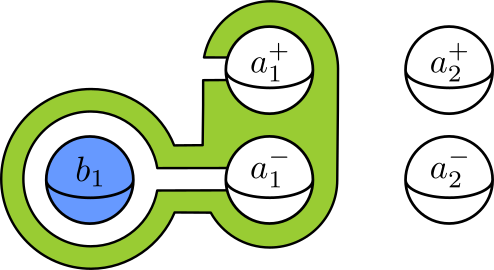
\includegraphics[width=\textwidth]{figures/sepconnect2.pdf}
        \caption{The conjugation $b_1 \mapsto a_1b_1a_1^{-1}$
        corresponds to pushing
        $b_1$ through $a_1^+$.}
        \label{fig:kput1}
    \end{subfigure}
    \caption{Nontrivial $\Gamma'_{n,s}$ generator actions on the base sphere $v$
    move $v$ at most distance 2 in $\mathcal S^{sep}_{n,s}$.}
    \label{sepconnect}
\end{figure}


Then $v'$ and $v$ are contained in a copy of $M_{1,2}$ bounded by $b_1$
and the sphere $u$ separating $a_1$ and $b_1$ from
$a_2, \ldots, a_n$ and $b_2, \ldots, b_s$.
If $n\geq 2$ or $s\geq 3$ we have that $u$
is essential and this gives a length 2 path $v$ to $u$ to $v'$ in $\mathcal {S}^{sep}_{n,s}$.
The inverse conjugation $b_1 \mapsto a_1^{-1}b_1a_1$ similarly
moves $v$ distance 2 in $\mathcal {S}^{sep}_{n,s}$.
Appealing to Putman's Lemma \ref{putmanlemma}, we conclude that
$\mathcal {S}^{sep}_{n,s}$ is connected for $n=1$ and $s\geq 3$.

Suppose $n \geq 2$.
Then generation of $\Gamma_{n,s}$ also requires transvection.
Consider the image $v'$ of $v$ under the
diffeomorphism corresponding to
the transvection $a_1 \mapsto a_1a_2^{-1}$,
as shown in orange in Figure \ref{sepconnect}.
Then $v'$ and $v$ are contained in a copy of $M_{2,1}$ bounded by
the sphere $u$ separating $a_1$ and $a_2$ from
$a_3, \ldots, a_n$ and $b_1, \ldots, b_s$.
If $n\geq 3$ or $s\geq 2$ we have that $u$
is essential and this gives a length 2 path $v$ to $u$ to $v'$ in $\mathcal {S}^{sep}_{n,s}$.
The inverse transvection $b_1 \mapsto a_1a_2$ similarly
moves $v$ distance 2 in $\mathcal {S}^{sep}_{n,s}$.
Appealing to Putman's Lemma \ref{putmanlemma}, we conclude that
$\mathcal {S}^{sep}_{n,s}$ is connected for $n=2$ and $s\geq 2$ or $n\geq 3$.




Finally, we show that $\mathcal {S}^{sep}_{2,1}$
is disconnected.
By capping the boundary component with a sphere we obtain a map
$$
\phi: \left (\mathcal {S}^{sep}_{2,1} \right )^{(0)} \to \left (\mathcal {S}^{sep}_{2,0} \right )^{(0)}
$$
Observe that if $u$ and $v$ are disjoint spheres of $\mathcal {S}^{sep}_{2,1}$
then $\phi(u)=\phi(v)$.
So $\phi$ gives a surjective simplicial map
$$
\mathcal {S}^{sep}_{2,1}  \to \mathcal {S}^{sep}_{2,0}.
$$
But as ${S}^{sep}_{2,0}$ is totally disconnected it must be that ${S}^{sep}_{2,1}$
is disconnected.
\end{proof}


\noindent
We say that a sphere is $M_n',s'$-bounding if it bounds an embedded copy of $M_{n',s'} \subset M_{n,s}$.

\begin{lemma}
  \label{sepgenpreserved}
For $k\leq n/2$,
$M_{k,1}$-bounding spheres are characteristic in $\mathcal {S}^{sep}_{n}$ for $n\geq 3$.
\end{lemma}
\begin{proof}
Suppose that $x \in \mathcal {S}^{sep}_{n}$ bounds
an $M_{k,1}$.
Observe the link of $x$ is isomorphic to
a join
$\mathcal S^{sep}_{k,1}  \ast \mathcal S^{sep}_{n-k,1}$.
By Lemma \ref{sepflagdim}
the dimensions of the sides of the join are $2k-3$ and $2n-2k-3$,
so any automorphism of $\mathcal {S}^{sep}_{n}$
must send $x$ to a genus $k$-bounding sphere.
\end{proof}


Observe that
$M_{1,0} = S_1 \times S_2$
so that $\pi_2(M_{1,0},p) \cong \Z$.
Using the long exact sequence of the pair
$(M_{1,1},\partial M_{1,1})$
we compute  $\pi_2(M_{1,0}) \cong \pi_2 (M_{1,1}, S^2 )$,
so $M_{1,1}$
contains a unique homotopy class of nonseparating sphere
generating the second homotopy group.

Then for any automorphism $\phi \in \aaut \left (  \mathcal S^{sep}_{n,s}\right)$
we can extend $\phi$ to a map
$\hat \phi : \mathcal S_{n,s} \to \mathcal S_{n,s}$.
If $x$ is a separating sphere we assign $\hat \phi (x) = \phi(x)$.
If $a$ is a nonseparating sphere, then
there is there is an $M_{1,1}$-bounding sphere $x$
bounding an $M_{1,1}$ which contains $a$.
Then $\phi(x)$ bounds an $M_{1,1}$ by
Lemma \ref{sepgenpreserved}.
We define $\hat \phi(a)$ to be
the nonseparating sphere in the $M_{1,1}$ bounded by $\phi(x)$.
We must first demonstrate that $\hat \phi$ is well defined.

Fix a nonseparating sphere $a$.
Define a \emph{sharing pair} $\{x,x'\}$ (sharing $a$) to be
$M_{1,1}$-bounding spheres $x$ and $x'$
such that $x$ and $x'$ each bound an $M_{1,1}$ containing $a$
and are contained in a common $M_{2,1}$ bounded by separating sphere $y$.

\begin{lemma}
  \label{sepsharepair}
If $\{x,x'\}$ is a sharing pair, then $\{\phi(x),\phi(x')\}$
is a sharing pair for any
automorphism $\phi \in \aaut\left( \mathcal S^{sep}_{n} \right )$.
\end{lemma}

\begin{proof}
Let $a_1$ be a nonseparating sphere of $M_{n,s}$
and let $\{x,x'\}$ be a sharing pair for $a_1$.
Then $x$ and $x'$ are adjacent to an $M_{2,1}$-bounding sphere $y$,
but not each other in $\mathcal S^{sep}_{n}$.
Let $a_2$ be a nonseparating sphere disjoint from $a1$ in the $M_{2,1}$ bounded by $y$.
Observe further we may find an $M_{1,1}$-bounding sphere
$z$ which intersects $y$, but not $x$ or $x'$.
\begin{figure}
% \floatbox[{\capbeside\thisfloatsetup{capbesideposition={right,top},capbesidewidth=.4\textwidth}}]{figure}[\FBwidth]
% {
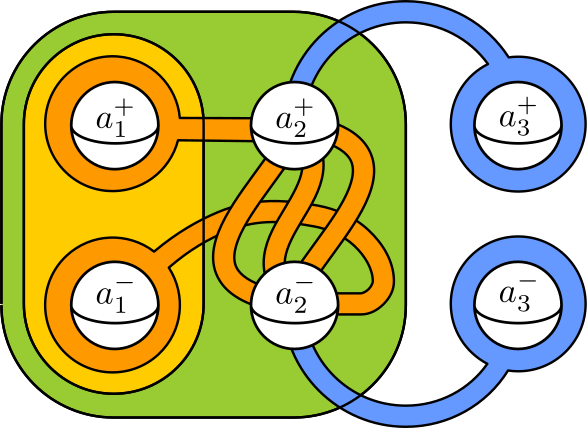
\includegraphics[width=.6\textwidth]{figures/sepsharepair.pdf}
\caption{
The sharing pair $x$ and $x'$ bound $M_{1,1}$ shown in yellow and orange.
They are contained in the green $M_{2,1}$ bounded by $y$.
The blue $M_{1,1}$ is bounded by $z$.
Observe an $M_{1,1}$-bounding sphere containing $a_1$ can be represented
by drawing two parallel copies $a^+_1$ and $a^-_1$ and then connecting them
by attaching a handle given by the regular neighborhood of an arc from $a_1^-$ to $a^+_1$ disjoint from $a_1$.
Fixing $a_1$, the spheres $x$ and $x'$ are determined by their respective intersection numbers with $a_2$.
}
\label{sepshare}
\end{figure}
Then, appealing to Lemma \ref{sepsharepair}, $\phi(x)$ and $\phi(x')$
must be intersecting $M_{1,1}$-bounding spheres.
Let $A$ be the $M_{2,1}$ bounded by $\phi(y)$.
$\phi(z)$ is disjoint from $\phi(x)$ and $\phi(x')$, but not $\phi(y)$.
Consider the image of $\phi(z)$ in the $A$.
If $\phi(z)$ bound a region containing a nonseparating sphere in
$A$, there would only be one class of separating sphere in $A$
disjoint from $\phi(z)$.
Then $\phi(z)$  must bound in $A$
a handle given by the boundary of a regular neighborhood of an arc of
$\pi_1(A,\partial A)$ which must pass through a nonseparating sphere $a$ of $A$.
But then $\phi(x)$ and $\phi(x')$ must both bound the nonseparating sphere of $A$ disjoint from $a$.
So $\{\phi(x),\phi(x')\}$ is a sharing pair.
\end{proof}

Let $a$ be a nonseparating sphere of $M_n$.
We will show that any two $M_{1,1}$-bounding spheres
which contain $a$ on their $M_{1,1}$-side are connected by a sequence of
sharing pairs.
Let $\mathcal P_a$ be the \emph{sharing pair} graph defined as follows.
The vertices of $\mathcal P_a$
are genus 1-bounding separating spheres of $M_n$ which
bound an $M_{1,1}$ containing $a$.
Two vertices of $\mathcal P_a$ are adjacent
if they form a sharing pair for $a$.

\begin{lemma}
  \label{seppairgraph}
The sharing pair graph $\mathcal P_a$ is connected.
\end{lemma}

\begin{proof}
We appeal to Putman's Lemma \ref{putmanlemma}
using the graph $X=\mathcal P_a$ and the group
$G \leq \Gamma_n$ fixing $a$ setwise.
Let $a_1, \ldots, a_n$ be a basis for $F_n$.
Then $G$ is generated by
diffeomorphisms corresponding to
permutations of $\{a_2, \ldots, a_n\}$,
inversions, and the transvections
$a_1 \mapsto a_1a^{-1}_2$ and $a_2 \mapsto a_2a^{-1}_3$.

Observe that $G$ acts transitively on
$M_{1,1}$-bounding spheres
which contain $a$ on their genus 1-side.
Let $v$ be the sphere separating
$a_1$ from $a_2, \ldots, a_n$.
Observe that of the chosen generators only
the transvection $\phi: a_1 \mapsto a_1a^{-1}_2$
has nontrivial action on $v$.
But, as can be seen in figure \ref{sepconnect},
 $v$ and $\phi(v)$
 are contained in an $M_{2,1}$
 so that  $\{ v, \phi(v) \}$ is a sharing pair.

 It follow by Putman's Lemma \ref{putmanlemma} that $\mathcal P_a$ is connected.
\end{proof}

The previous Lemma shows that $\hat \phi$ is well defined.
If $a$ is a nonseparating sphere of $M_n$
and $x$ and $x'$ $M_{1,1}$-bounding sphere bounding an $M_{1,1}$ containing $a$,
then as $P_a$ is connected there is a sequence of sharing pairs from $x$ to $x'$.
By Lemma \ref{sepsharepair} this gives a sequence of
sharing pairs from $\phi(x)$ to $\phi(x')$.
But then $\phi(x)$ and $\phi(x')$ share the same nonseparating sphere
so that $\hat \phi (a)$ is well defined.

Certainly $\hat \phi$ is simplicial.
If $a$ and $a'$ are disjoint nonseparating spheres
then there are disjoint $M_{1,1}$-bounding spheres $x$ and $x'$ bounding
disjoint copies of $M_{1,1}$ separating $a$ and $a'$, respectively.
Since $\phi(x)$ and $\phi(x')$ are disjoint $M_{1,1}$-bounding spheres,
$\hat \phi(a)$ and $\hat \phi(a')$ are also disjoint.
If $y$ is a separating sphere disjoint from $a$, then
either there is an $M_{1,1}$-bounding sphere separating $a$ from $y$
or $y$ is an $M_{1,1}$-bounding sphere, so that $\hat \phi(a)$ is disjoint from $\hat \phi (y) = \phi(y)$.

\begin{theorem}[Proposition]
  The natural map $\oout (F_n) \to \aaut \left ( \mathcal S^{sep}_n \right)$
  is an isomorphism for $n \geq 3$.
  \label{thm:sep}
\end{theorem}

\begin{proof}
The map constructed above
$$\Phi: \aaut \left ( \mathcal S^{sep}_n \right) \to \aaut \left ( \mathcal S_n \right)$$
with $\phi \mapsto \hat \phi$
is an isomorphism with the  map simply restricting automorphisms
$$\aaut \left ( \mathcal S_n \right) \to   \aaut \left ( \mathcal S^{sep}_n \right)$$
giving an inverse to $\Phi$.
Then the result follows from
Theorem \ref{aramsouto}.
\end{proof}

\section{Complexes of High Genus Separating Spheres}

For $k\leq n/2$, we call a sphere $x \in [S^2, M_{n,s}]$ $k$-separating
if both components of
$M_{n,s}-x$
contain either a boundary component
or at least $k$ disjoint separating spheres.
If $x$ bounds a copy of $M_{j,1}$ with $j<n/2$,
we refer to it as to as $x^{in}$, or the \emph{inside} of $x$.
We will also describe objects disjoint from and inside of $x$ as \emph{engulfed} by $x$,
and disjoint objects on the outside as \emph{exgulfed} by $x$.

Let $\mathcal S^{sep,k}_{n,s} \subset \mathcal S^{sep}_{n,s}$
be the subcomplex spanned by homotopy classes of essential $k$-separating
spheres.

Observe that for $k>1$,
$\mathcal S^{sep,k}_{n,s}$
does not have a uniform dimension.
For example, in the case with no boundary components, $s=0$,
we can construct
a maximal (with respect to inclusion)
simplex of maximal dimension
\hbox{$n-2k$}
as in Figure \ref{bigsimp}.
\begin{figure}[b!]
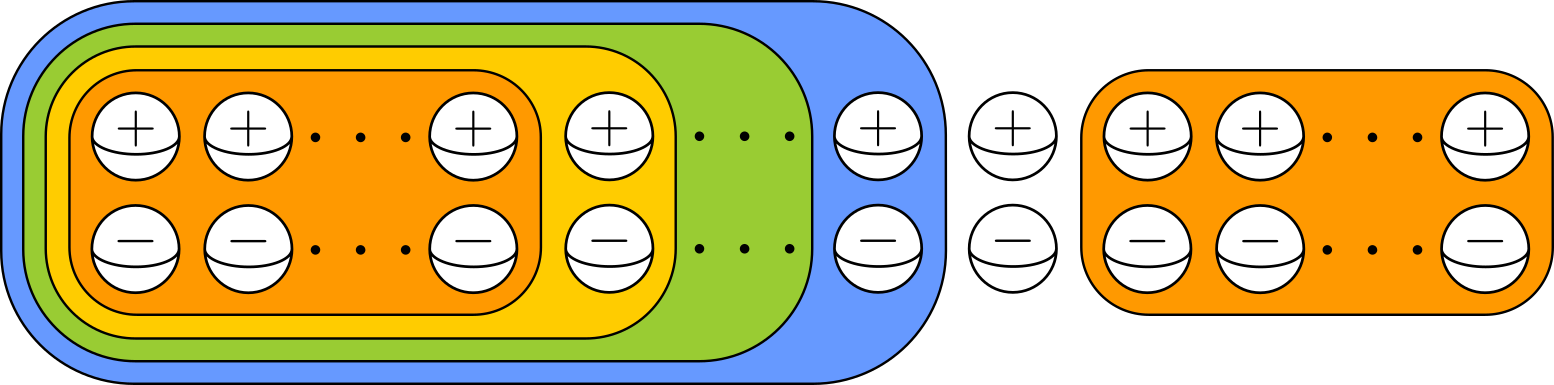
\includegraphics[width=\textwidth]{figures/bigsimplex.pdf}
\caption{A maximal dimension maximal simplex of $\mathcal S^{sep,k}_{n}$ for $k>1$
is spanned by $n-2k+1$ spheres and cuts $M_n$ into 2 copies of $M_{k,1}$ and $n-2k$
copies of $M_{1,2}$.
The corresponding graph of $M_{n}$ components is an unbranched tree
with 2 leaves of weight $k$ and $n-2k$ internal vertices of weight 1.}
\label{bigsimp}
\end{figure}
If we write $n=qk+r$ by Euclidean division,
then we can construct maximal (with respect to inclusion) simplices
of smaller dimension $2q+r-4$ as in Figure \ref{lilsimp}.
\begin{figure}[b!]
\includegraphics[width=\textwidth]{figures/smallersimplex.pdf}
\caption{A minimal dimension maximal simplex of $\mathcal S^{sep,k}_{n}$ for $k>1$
is spanned by $2q+r-3$ spheres and cuts $M_n$
into $q$ copies of $M_{k,1}$ and $r$ copies of $M_{1,2}$ and $q-2$ copies of $M_{0,3}$.
The corresponding graph of $M_{n}$ components is a tree
with $q$ leaves of weight $k$ and $q-2$ internal vertices weight 0
and $r$ internal vertices of weight 1.}
\label{lilsimp}
\end{figure}

If there are boundary spheres we can construct a maximal dimension simplex
similar to Figure \ref{bigsimp}
by replacing the $M_{k,1}$-bounding spheres with boundary spheres.
Similar linear nesting shows any $k$-separating sphere can be contained in a maximum dimension simplex
of dimension for $k>1$
$$
\max_n \left \{
\Delta^n \hookrightarrow
\mathcal S^{sep,k}_{n,s}
\right \}
=
\begin{cases}
  n-2k & \mbox{ if } s=0\\
  n-k & \mbox{ if } s=1\\
  n+s-3 & \mbox{ if } s\geq 2
\end{cases}.
$$

\begin{lemma}
  \label{ksepconnect}
For $1<k<n/2$,
the complex of $k$-separating spheres
$\mathcal S^{sep,k}_{n,s}$
is connected whenever it has positive dimensional simplices if $s=0$,
and whenever it has 2 dimensional simplices if $s>0$.
\end{lemma}

\begin{proof}
The proof is similar to the proof of Lemma \ref{}!!!!,
utilizing Putnam's Lemma with the group $\Gamma'_{n,s}$.

Consider first the case with $s=0$
and suppose that $\mathcal S^{sep,k}_{n,s}$ has positive dimensional simplices.
So $n>2k$, and in particular
there are $M_{k,1}$ and $M_{k+1,1}$-bounding spheres in $\mathcal S^{sep,k}_{n,s}$.
Choose a sphere $v$ to be an $M_{k,1}$-bounding sphere.
Observe that every $k$-separating sphere is disjoint from a
$M_{k,1}$-bounding sphere, and the $M_{k,1}$-bounding spheres
are exactly the $\Gamma_n$ orbit of $v$.
Let $a_1,\ldots,a_n$ be a maximal collection of disjoint non-separating spheres
of $M_{n}$ with $a_1,\ldots, a_k$ engulfed by $v$.
Consider as a generating set for $\Gamma_n$
the transpositions and inversions of $a_1,\ldots,a_n$
and the transposition diffeomorphism $t$ corresponding to $a_1 \mapsto a_1a_{k+1}^{-1}$.
Observe that every inversion fixes $v$.
Observe that a transposition $\phi$ either fixes $v$, in the case it swaps
spheres on the same side of $M_n-v$, or $\phi(v)$ and $v$ are contained in a common
$M_{k+1,1}$-bounding sphere which is $k$-separating, as in Figure
\ref{fig:kput0}.
Finally, $v$ and $t(v)$ are contained in a common
$M_{k+1,1}$-bounding sphere as in Figure \ref{fig:kput1}.
The connectivity then follows by Putnam's Lemma.
\begin{figure}[b!]
    \centering
    \begin{subfigure}[b]{0.4\textwidth}
        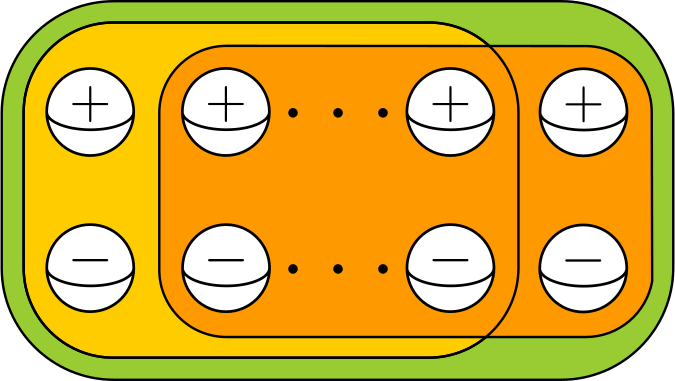
\includegraphics[width=\textwidth]{figures/kput0.pdf}
        \caption{Transpositions move $M_{k,1}$-bounding spheres distance 2.}
        \label{fig:kput0}
    \end{subfigure}
    ~
    \begin{subfigure}[b]{0.4\textwidth}
        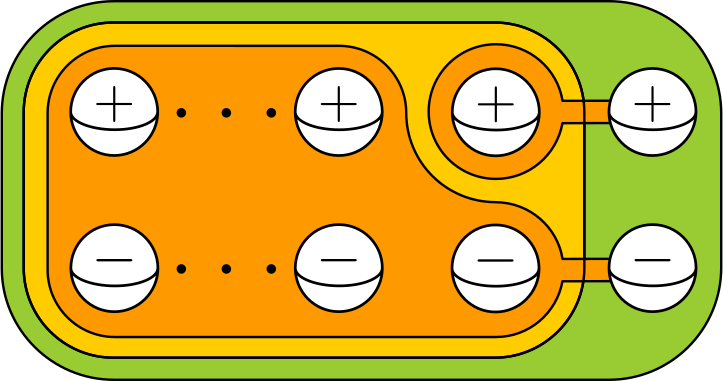
\includegraphics[width=\textwidth]{figures/kput1.pdf}
        \caption{Transvections move $M_{k,1}$-bounding spheres distance 2.}
        \label{fig:kput1}
    \end{subfigure}
    \caption{Nontrivial $\Gamma_n$ generator actions on the base sphere $v$
    move $v$ at most distance 2 in $\mathcal S^{sep,k}_{n,s}$.}
    \label{fig:kput01}
\end{figure}

Consider the case with $s>0$.
If
$s=1$
then to have dimension 2 simplices $n \geq k+2$,
and $M_{2,2}$-bounding spheres are $k$-separating.
If
$s>1$
then to have dimension 2 simplices $n+s\geq 5$.
If $s=1$ then $n \geq 4$
so that $M_{2,2}$-bounding spheres are disjoint from a
$M_{k,1}$-bounding sphere and must be $k-separating$.
If $s>1$ then $n \geq 4$
so that $M_{1,3}$ and $M_{2,2}$-bounding spheres are disjoint from a
$M_{1,2}$ or $M_{k,1}$-bounding sphere and must be $k-separating$.


Choose a sphere $v$ to be an $M_{1,2}$-bounding sphere.
Observe that every $k$-separating sphere is disjoint from a
$M_{1,2}$-bounding sphere, and the $M_{1,2}$-bounding spheres
are exactly the $\Gamma'_{n,s}$ orbit of $v$.
Let $b_1,\ldots,b_s$ be the bounding spheres
and let $a_1$ be a nonseparating sphere engulfed by $v$ and $a_2, \ldots, a_n$
disjoint nonseparating spheres disjoint from $v$ and $a_1$.
Consider as a generating set for $\Gamma'_{n,s}$
diffeomorphisms corresponding to
transpositions of $a_1,\ldots,a_n$,
transpositions of $b_1,\ldots,b_s$,
$t$ the transvection $a_1 \mapsto a_1a_2^{-1}$,
and $u$ the $b_1$ push corresponding to
conjugation $b_1 \mapsto a_1b_1a_1^{-1}$.
Observe first that $u$ leaves $v$ fixed.
Observe  that $\phi$ a
transposition of  $a_1,\ldots,a_n$
either leaves $v$ if it fixes $a_1$, or
swaps $a_1$, and then $\phi(v)$ and $v$
are engulfed by an $M_{2,2}$-bounding sphere as in Figure \ref{fig:kput2}.
Observe that $\psi$ a
transposition of  $b_1,\ldots,b_s$
either leaves $v$ if it fixes $b_1$, or
swaps $b_1$, and then $\psi(v)$ and $v$
are engulfed by an $M_{1,3}$-bounding sphere as in Figure \ref{fig:kput3}.
Finally,
$v$ and $t(v)$
are engulfed by an $M_{2,2}$-bounding sphere as in Figure \ref{fig:kput4}.
The connectivity then follows by Putnam's Lemma.
\begin{figure}[b!]
    \centering
    \begin{subfigure}[b]{0.3\textwidth}
        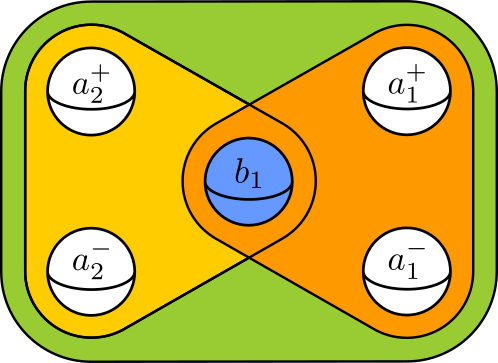
\includegraphics[width=\textwidth]{figures/kput2.pdf}
        \caption{$a$-Transposition}
        \label{fig:kput2}
    \end{subfigure}
    ~
    \begin{subfigure}[b]{0.3\textwidth}
        \includegraphics[width=\textwidth]{figures/kput3.pdf}
        \caption{$b$-Transposition}
        \label{fig:kput3}
    \end{subfigure}
    ~ %add desired spacing between images, e. g. ~, \quad, \qquad, \hfill etc.
      %(or a blank line to force the subfigure onto a new line)
    \begin{subfigure}[b]{0.3\textwidth}
        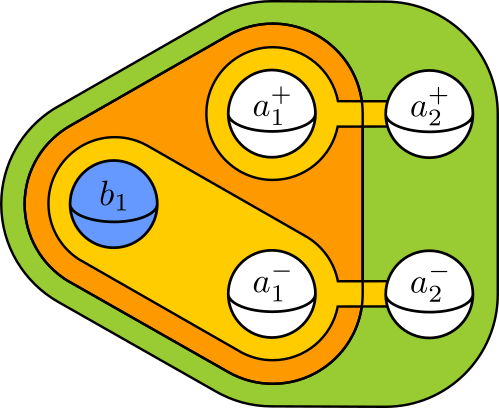
\includegraphics[width=\textwidth]{figures/kput4.pdf}
        \caption{Transvection}
        \label{fig:kput4}
    \end{subfigure}
    \caption{Nontrivial $\Gamma'_{n,s}$ generator actions on the
    base sphere $v$ move $v$ at most distance 2
    in $\mathcal S^{sep,k}_{n,s}$.}
    \label{fig:kput234}
\end{figure}
\end{proof}

\begin{lemma}
Let $n\geq 3$ and $\phi \in \aaut{ \left ( \mathcal S^{sep,k}_{n} \right ) }$.
For $n/2>j\geq k$,
if $x$ is a
$M_{j,1}$-bounding spheres
engulfing a sphere $y$,
then $\phi(x)$
is a
$M_{j,1}$-bounding spheres
engulfing the sphere $\phi(y)$.
\label{kengulfschar}
\end{lemma}

\begin{proof}
  Suppose that $x$ bounds an $M_{j,1}$ in $\mathcal S^{sep,k}_{n}$.
  Consider the subcomplex
  $\mathcal E_x$ spanned by spheres engulfed by $x$
  and the subcomplex
  $\mathcal F_x$ spanned by spheres disjoint but not engulfed by $x$.
  The link of $x$ is a join $\mathcal E_x \ast \mathcal F_x$
  and
  $\mathcal E_x \cong \mathcal S^{sep,k}_{j,1}$
  and $\mathcal F_x \cong \mathcal S^{sep,k}_{n-j,1}$.
  Then according to Lemma \ref{ksepconnect},
  $\mathcal E_x$
  and $\mathcal F_x$
  have simplices with maximal dimension
  $j-k$ and $n-j-k$, respectively.
  So the link of $\phi(x)$ must have the same structure
  and $\phi(x)$ must be $M_{j,1}$-bounding.
  Note that since
  $$\phi \left( \mathcal E_x \right) =\mathcal E_{\phi(x)}$$
  any sphere $y$ engulfed by $x$ has $\phi(y)$ engulfed by $\phi(x)$.
\end{proof}

We hope to extend automorphisms of
$\mathcal S^{sep,k}_{n}$ to
automorphisms of $\mathcal S^{sep,k-1}_{n}$
by
a
combinatorial characterization of
$M_{k-1,1}$-bounding spheres in $\mathcal S^{sep,k}_{n}$.

This is the direct analog of handle pairs of \ref{}METACONJECTURE!!!!
\begin{definition}
  If $x$ is a $M_{k,1}$-bounding sphere engulfed by $M_{k+1,1}$-bounding sphere $y$
  we say that a pair $v,w$ of $M_{k,1}$-bounding spheres
  \emph{carve} $x$ from $y$ if
  \begin{enumerate}[(1)]
    \item Each pair of $v,w,y$ intersects, but $v,w,y$ are all disjoint from $x$.
    $$
    \begin{tikzcd}[every arrow/.append style={dash}]
      v \arrow{r} & x \arrow{r} & y\\
      w \arrow{ur} &&
    \end{tikzcd}
    $$
    \item The $M_{k,1}$-bounding sphere $x$ is the unique sphere engulfed by $y$
    and disjoint from both $v$ and $w$.
    \item There is more than one $M_{k,1}$-bounding sphere engulfed by $y$ and disjoint
    from $v$ but not $w$.
    \item There is more than one $M_{k,1}$-bounding sphere engulfed by $y$ and disjoint
    from $w$ but not $v$.
  \end{enumerate}
\end{definition}

It follows immediately from this combinatorial definition and
Lemma \ref{kengulfschar} that carving is characteristic.
The following Lemma shows additionally that there is
a unique non-separating sphere which was
``carved away'' from $y$.


\begin{lemma}
  Let $\phi \in \aaut \mathcal S^{sep,k}_{n}$.
  If $v,w$ carve $x$ from $y$,
  then
  \begin{enumerate}[(1)]
  \item $\phi(v), \phi(w)$ carve $\phi(x)$ from $\phi(y)$
  \item One of the spheres $v$ or $w$
  contains a disk or annulus $s$ with $\partial s \subset y$ whose image in $y^{in}/y$
  is homotopic to a nonseparating sphere.
  \item There is an arc $\alpha$ with endpoints on $y$
  such that $v$ and $w$ separate $\alpha$ from $x$.
  \item $x$ is the unique $M_{k,1}$-bounding sphere engulfed by $y$ and disjoint from $s$ and $\alpha$.
\end{enumerate}
\label{carvingchar}
\end{lemma}

\begin{proof}
  (1) follows from Lemma \ref{kengulfschar} and the combinatorial definition of carving.\\
  (2) Fix representatives for $v$, $w$, $x$, and $y$ which intersect minimally and transversely.
  Then $w\cap y^{in}$ is a collection of disks and annuli with boundary on $y$.
  No component disk or annulus of $w\cap y^{in}$ can be separating,
  or else there would be at most $M_{k,1}$ in $y^{in}$
  disjoint from $w$.
  Similarly $v\cap y^{in}$ is a collection of disks and annuli, no one of which separates $y^{in}$.
  Let $\beta$ be any nontrivial loop in $y^{in}-x^{in}$ and based at
  a point on $x$.
  Then $\beta$ must intersect either $v$ or $w$, or else
  the pushes of any nonseparating sphere of $x$ about $\alpha$
  would yield infinitely many $M_{k,1}$-bounding spheres engulfed by $y$
  and disjoint from $v$ and $w$, contrary to the hypothesis.
  Since no such $\beta$ exists,
  there must a component $s$ of $v\cap y^{in}$ or $w\cap y^{in}$
  whose image in the quotient
  $y^{in}/y$ is homotopic to a nonseparating sphere.\\
  (3) Let $a$ be a nonseparating sphere engulfed by $y$ and exgulfed by $x$
  and disjoint from the nonseparating component $s$ as above.
  If $v\cap y^{in}$ or $w\cap y^{in}$
  have a component which intersects $a$, then as $v$ and $w$ are separating there
  must be an arc intersecting $a$ with endpoints on $y$ which they separate from $x$.
  Suppose that $v$ and $w$ are disjoint from $a$.
  If there is a loop $\gamma$ based at $a$ which winds through a noseparating sphere engulfed by $x$
  and is disjoint from $v$ and $w$,
  then the pushes of $a$ along $\gamma$ leave $v$ and $w$ unchanged,
  but the images of $x$ give infintely many $M_{k,1}$-bounding spheres
  engulfed by $y$ and disjoint from $v$ and $w$, in contradiction
  with the definiton of carving.
  Then $v$ and $w$ must separate $a$ from $x$ in $y$, and there is an
  arc $\alpha$ with end points on $y$ which intersects $a$ once and
  so must be separated from $x$ by $v$ and $w$.\\
  (4) Assume to the contrary there is some $x'$ engulfed by $y$,
   distinct from $x$,
   and disjoint from $s$ and $\alpha$.
   Then there must be some nonseparating sphere $a$ engulfed $x'$ but not $x$.
   Note that $y^{in}-x^{in} \cong M_{1,2}$
   and consider the components of $a \cap (y^{in}-x^{in})$.
   If $a \cap (y^{in}-x^{in})$ has a nonseparating disk,
   it must intersect $\alpha$.
   If $a \cap (y^{in}-x^{in})$ contains a nontrivial arc,
   it must intersect $s$. So $a$ must be engulfed by $x$.
\end{proof}

\begin{definition}
Define a $M_{k-1,1}$-sharing pair
 $\{x_0,x_1\}$
 to be a pair of $M_{k,1}$-bounding spheres $x_0,x_1 \in \mathcal S^{sep,k}_{n}$
such that:
\begin{enumerate}[(1)]
  \item
  There are $M_{k,1}$-bounding spheres $x_2,x_3$ and a
$M_{k+1,1}$-bounding sphere $y$
such that the induced subgraph of $\mathcal S^{sep,k}_{n}$
on $y,x_0,x_1,v_0,v_1,w_0,w_1$ is exactly
$$
\begin{tikzcd}[every arrow/.append style={dash}]
x_0 \arrow{d} \arrow{r} \arrow[bend right=60]{dd}& y \arrow{r}& x_1 \arrow{d} \arrow[bend left=60]{dd}\\
v_0 \arrow{rr} \arrow{rrd}&&  v_1\\
w_0 \arrow{rr} \arrow{rru} &&  w_1
\end{tikzcd}
$$
and
\item For $i=0,1$ the spheres $v_i,w_i$ carve $x_i$ from $y_i$.
\item For $z_0 \in \{v_0,w_0\}$ and $z_1 \in \{v_1,w_1\}$,
there is no $M_{k,1}$-bounding sphere engulfed by $y$ and disjoint from both
$z_0$ and $z_1$.
\end{enumerate}
\label{def:ksharepair}
\end{definition}


\begin{lemma}
  The spheres of an $M_{k-1,1}$-sharing pair
  uniquely engulf a
  $M_{k-1,1}$-bounding sphere in $M_n$.
\end{lemma}

\begin{proof}
Let $\{x_0,x_1\}$ be a sharing pair with $y,v_0,w_0,v_1,w_1$ as above.
Let $s_i$ and $\alpha_i$
be as specified in Lemma \ref{carvingchar},
so that,
without loss of generality,
$s_i$ is a component of $v_i \cap y^{in}$ which is nonseparating in $y$.
And $\alpha_i$ is a loop with endpoints on $y$ which $v_i$ and $w_i$ separate from $x_i$.
But as $v_0$ and $v_1$ are disjoint, so are $s_0$ and $s_1$.

Since there is no $M_{k,1}$-bounding sphere disjoint from
both $v_0$ and $v_1$, it must be no $M_{k-1,1}$-bounding sphere
is disjoint from both $s_0$ and $s_1$ or from both $\alpha_0$ and $\alpha_1$.

Then $\alpha_1$ must intersect $x_0$,
and there are $k-1$
disjoint nonseparting spheres $a_1,\ldots, a_{k-1}$
engulfed by $x$ and disjoint from $\alpha_1$.


Consider the images in $y^{in}/y \cong M_{k+1,1}$.
Then the images of $s_0$ and ${s_1}$
are distinct nonseparating spheres in $y^{in}/y$.
Further since there is no $M_{k,1}$-bounding sphere disjoint from
both, forgetting the basepoint $y/y$ in $y^{in}/y$
gives distinct, disjoint spheres
$\overline{s_0}$ and $\overline{s_1}$ of $y^{in}$.
Let $\Sigma$ be a system of $n-k-1$ disjoint spheres exgulfed by $y$.

The let $z$ be the unique sphere separating
$a_1,\ldots,a_k$ from $\overline{s_0}$, $\overline{s_1}$, and $\Sigma$.
Then $z$ is $M_{k-1,1}$-bounding and
uniquely engulfed by both $x_0$ and $x_1$.
\end{proof}


\begin{lemma}
  Sharing pairs are characteristic.\\
  If $\{x_0,x_1\}$ is an $M_{k-1,1}$-sharing pair with $x_0,x_1 \in \mathcal S^{sep,k}_n$
  and $\phi \in \aaut \mathcal S^{sep,k}_n$,
  then $\{\phi(x_0),\phi(x_1)\}$ is an $M_{k-1,1}$-sharing pair.
  \label{lemma:sharepreserve}
\end{lemma}

\begin{proof}
  Let $y,x_0,v_0,w_0,x_1,v_1,w_1$ be as in Definition \ref{def:ksharepair}.
  By Lemma \ref{kengulfschar} $\phi(x_0),\ldots, \phi(x_3)$
  are $M_{k,1}$-bounding and $\phi(y)$ is $M_{k+1,1}$-bounding.
  The $\phi$ image of the induced subgraph on $y,x_0,v_0,w_0,x_1,v_1,w_1$
  is an isomorphic graph.
  Property (2) is preserved by Lemma \ref{carvingchar}.
  Property (3) of Definition \ref{def:ksharepair}
  is preserved by its combinatorial definition.
\end{proof}

Although the representation of $M_{k-1,1}$-bounding spheres
are

\begin{lemma}
  Every $M_{k-1,1}$-bounding sphere $x$ admits an $M_{k-1,1}$-sharing pair in
  $\mathcal S^{sep,k}_{n}$ engulfing $x$, provided $n\geq 3k$.
  \label{lemma:ksharexist}
\end{lemma}

\begin{proof}
  By a change of coordinates the,
  arrangement in Figure \ref{fig:ksharing} shows a possible pair sharing $x$.

  \begin{figure}[h!]
  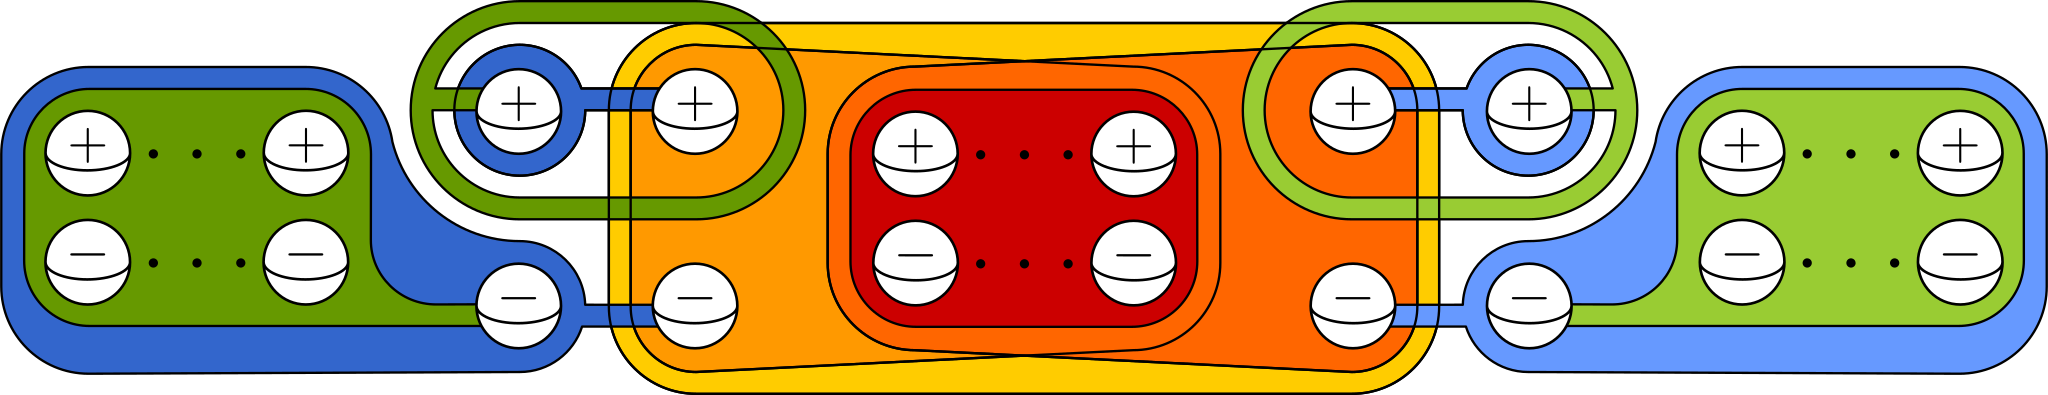
\includegraphics[width=\textwidth]{figures/ksharingnotpent.pdf}
  \caption{
    A sharing pair and the requisite carvings.
    The pair $\{x_0,x_1\}$ is shown bounding dark and light orange, respectively.
    The pair shares the $M_{k-1,1}$-bounding sphere $x$ shown bounding red.
    The pair is engulfed by $M_{k+1,1}$-bounding sphere $y$ shown in yellow.
    Dark orange $x_0$ is carved by $v_0$ and $w_0$ shown in dark green and blue.
    Light orange $x_1$ is carved by $v_1$ and $w_1$ shown in light green and blue.
  }
  \label{fig:ksharing}
  \end{figure}
\end{proof}


We call three spheres an $M_{k-1,1}$-sharing triple if
the spheres pairwise form sharing pairs and all engulf
a common $M_{k-1,1}$-bounding sphere.

\begin{lemma}
  Sharing triples are characteristic.\\
  If $\{x_0,x_1,x_2\}$ is an $M_{k-1,1}$-sharing triple with $x_0,x_1,x_2 \in \mathcal S^{sep,k}_n$
  and $\phi \in \aaut \mathcal S^{sep,k}_n$,
  then $\{\phi(x_0),\phi(x_1),\phi(x_2)\}$ is an $M_{k-1,1}$-sharing triple.
  \label{lemma:sharetrippreserve}
\end{lemma}

\begin{proof}
  According to Lemma \ref{lemma:sharepreserve}
  if $x_0,x_1,x_2$ pairwise form sharing pairs,
  then so do $\phi(x_0),\phi(x_1),\phi(x_2)$.
  It remains only to see that
  $\phi(x_0),\phi(x_1),\phi(x_2)$ all engulf a
  common $M_{k-1,1}$-bounding sphere, rather that a distinct
  $M_{k-1,1}$-bounding sphere for each pair.
  We reduce the proof to showing
  $\phi(x_0),\phi(x_1),\phi(x_2)$ all engulf a
  common $M_{k-1,1}$-bounding sphere if and only if there is
  no $M_{k+1,1}$-bounding sphere $y$ engulfing
  $\phi(x_0),\phi(x_1),$ and $\phi(x_2)$.
  Then if there were a $y$ engulfing $\phi(x_0),\phi(x_1),$ and $\phi(x_2)$,
  $\phi^{-1}(y)$ engulfs $x_0,x_1,x_2$, which would contradict that
  $\{x_0,x_1,x_2\}$ is a sharing triple.

  Observe that, as in the proof of Lemma \ref{lemma:sharepreserve},
  since $\phi(x_0),\phi(x_1),\phi(x_2)$
  are pairwise sharing pairs,
  there are three pairwise-disjoint $M_{1,1}$-bounding spheres $z_0,z_1,z_2$
  such that $z_i$ is uniquely engulfed by $\phi(x_i)$ and disjoint
  but not engulfed by $\phi(x_{i+1})$, for $i \in \Z/3$.
  The sphere shared by $\{\phi(x_i),\phi(x_{i+1})\}$
  is in $\phi(x_i)^{in}-z_i^{in}$.
  If $\phi(x_0),\phi(x_1),\phi(x_2)$ all engulf a
  common $M_{k-1,1}$-bounding sphere $x$,
  then any sphere engulfing $\phi(x_0),\phi(x_1),\phi(x_2)$
  contains $x,z_0,z_1,$ and $z_2$ so must be $M_{j,1}$-bounding for $j\geq k+2$.
  If $\phi(x_0),\phi(x_1),\phi(x_2)$ do not engulf
  a common $M_{k-1,1}$-bounding sphere,
  then for $i \in \Z/3$
  we have a distinct $M_{k-1,1}$-bounding sphere
  shared by
  $\{\phi(x_i),\phi(x_{i+1})\}$ and which engulfs $z_{i-1}$.
  But then
  $\phi(x_0),\phi(x_1),\phi(x_2)$ do all engulf
  a common $M_{k-2,1}$-bounding sphere $x$
  such that $\phi(x_i)$ engulfs $x$ and $z_i$ and $z_{i+1}$.
  Then the same $M_{k+1,1}$-bounding sphere $y$ fits into the defining pentagon
  of Definition \ref{def:ksharepair}
  for all three sharing pairs.
\end{proof}

Let $x$ be an $M_{k-1,1}$-bounding sphere.
We will show that any two sharing pairs engulfing $x$
are connected by a sequence of sharing triples.
Let $\mathcal P_x$ be the \emph{sharing pair} graph defined as follows.
The vertices of $\mathcal P_x$ are $M_{k-1,1}$-sharing pairs in
$\mathcal S^{sep,k}_n$ engulfing
$x$, where $n\geq 3k$.
Two vertices $\{x_0,x_1\}$ and $\{x_1,x_2\}$
of $\mathcal P_x$ are adjacent if the pairs
have a common member and the three spheres
form an $M_{k-1,1}$-sharing triple engulfing $x$.

% By Lemma \ref{lemma:sharepreserve}, an automorphism
% $\phi \in \aaut \mathcal S^{sep,k}_n$
% induces an isomorphism
% $\mathcal P_x \stackrel{\cong}{\longrightarrow} \mathcal P_{\phi(x)}$
% .


\begin{lemma}
  The sharing pair graph $\mathcal P_x$ is connected for $n\geq 3k$ and $k\geq 2$.
  \label{lem:kshareconnect}
\end{lemma}

\begin{proof}
  We appeal to Putman's Lemma \ref{putmanlemma}.
  Fix an $M_{k-1,1}$-bounding sphere $x$ and
  an $M_{k-1,1}$-sharing pair $v=\{x_0,x_1\}$ engulfing $x$ with $x_0$ and $x_1$ having geometric intersection 1.
  Let $G \leq \Gamma_n$ be the subgroup fixing $x^{in}$, so that $G\cong \Gamma_{n-k+1,1}$.


  Observe that if two $x$-sharing pairs $\{x_0,x_1\}$ and $\{x_1,x_2\}$
  contain a common member $x_1$ and with all three spheres engulfed
  by a common $M_{k+1,1}$-bounding sphere $y$,
  then we can find a length 2 path in $\mathcal P_x$
  by choosing $x_3$ with intersection 1 with $y$
  and engulfing an $M_{1,1}$-bounding sphere which is disjoint from $y$.
  Then $\{x_0,x_1,x_3\}$ and $\{x_1,x_2,x_3\}$ are sharing triples, since
  they are pairwise sharing pairs and all engulf $x$.
  So if $y_0$ is the $M_{k+1,1}$-bounding sphere engulfing $v=\{x_0,x_1\}$,
  and
  $\{x'_0,x'_1\}$ is any sharing pair
  engulfed by $y'_0$,
  then there is $g \in G$ such that $g(x_1)= x'_1$ and $g(y_0) = y'_0$.
  So the orbit $G\cdot v$ is at most distance 2 from any sharing pair vertex of $\mathcal P_x$.
  This completes the first criterion of Putnam's Lemma \ref{putmanlemma}.


  Fix a system of nonseparating spheres
  $a_0, \ldots, a_{n-k}$ disjoint and not engulfed by $x$
  with $a_0$ but not $a_{n-k}$ engulfed by $x_0$ and $a_{n-k}$ but not $a_0$ engulfed by $x_1$.
  Then $G\cong \aaut \langle a_0,\ldots ,a_{n-k}, \rangle $
  is generated by diffeomorphism classes
  corresponding to
  inversions of $a_0, \ldots, a_{n-k}$ (though these always fix $v$),
  transpositions  of $a_0, \ldots, a_{n-k}$
  the transvection $t':a_0 \mapsto a_0a_1^{-1}$.

  \begin{figure}[b!]
    \centering
          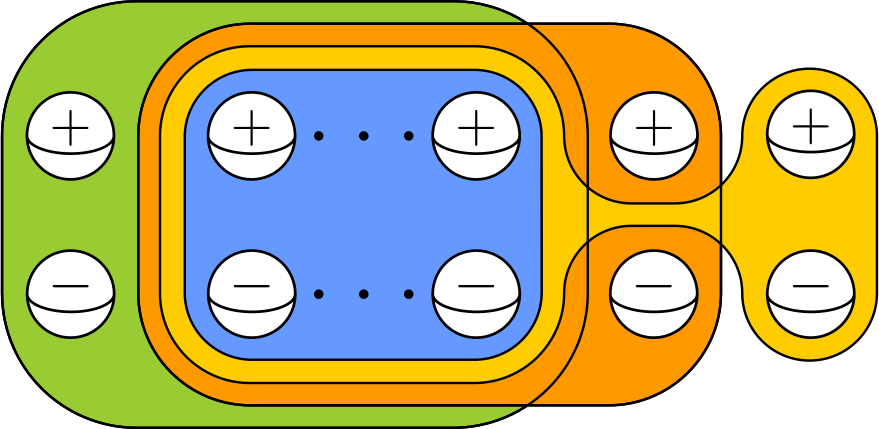
\includegraphics[width=.7\textwidth]{figures/ksharepairgraph0.pdf}
          \caption{
          The sharing pair $v$ is formed by the  green $x_1$ and  orange $x_0$ spheres.
          Transpositions move the sharing pair $v$ either distance 0 in $\mathcal P_x$,
          by swapping orange and green, or
          distance 1, by, for example, swapping orange and yellow.
          Observe that the orange, yellow, and green $M_{k,1}$-bounding spheres form a sharing
          triple for the blue sphere $x$.}
          \label{fig:ksharepair0}
  \end{figure}



  Consider first the action of   transpositions $t$ on
  the sharing pair $v \in \mathcal P_x$.
  If neither $a_0$ nor $a_{n-k}$ are swapped by $t$,
  then the sharing pair $v$ is fixed.
  If both $a_0$ and $a_{n-k}$ are swapped by $t$,
  then $x_0$ and $x_1$ are swapped, so that the sharing pair $v=\{x_0,x_1\}$
  is still fixed.
  If exactly one of $a_0$ or $a_{n-k}$ is swapped by $t$
  transposition then exactly one of $x_0$, $x_1$ are exchanged from the sharing pair,
  so that the transposition action moves the sharing pair $v$ distance 1 in $\mathcal P_x$,
  as shown in Figure \ref{fig:ksharepair0}.


  \begin{figure}[t!]
    \centering
          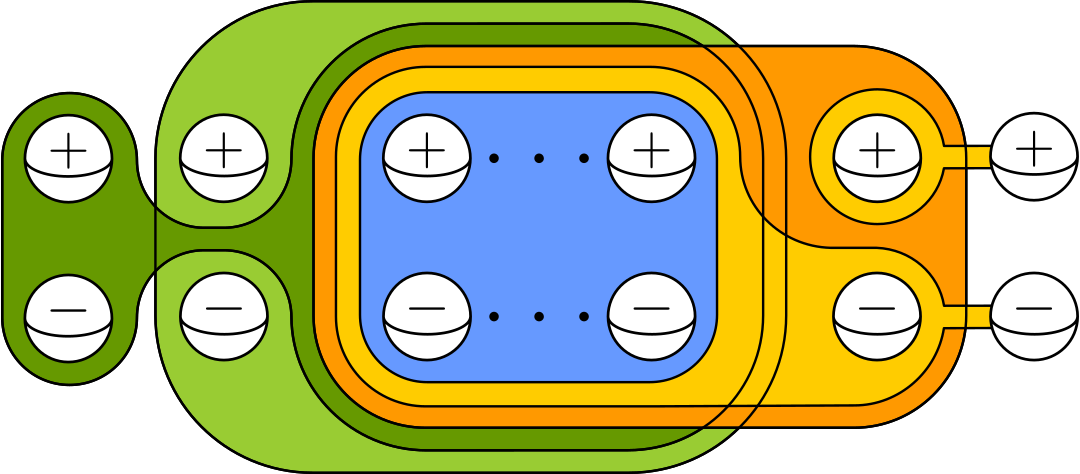
\includegraphics[width=.8\textwidth]{figures/ksharepairgraph1.pdf}
          \caption{The chosen transvection moves $v$
          distance 2 in $\mathcal P_x$.
          Observe that $x_0$ orange, $x_1$ light green,
          $x_2$ dark green, and $t'(x_0)$ yellow can be organized
          into two sharing triples: orange with the greens and yellow with the greens.}
          \label{fig:ksharepair1}
  \end{figure}

  Finally consider the transvection action $t':a_0 \mapsto a_0a_1^{-1}$ on $\mathcal P_x$.
Then $t'(x_0)$ (shown in yellow in Figure \ref{fig:ksharepair1})
intersects $x_0$ (shown in orange) twice and $t'(x_1)=x_1$ (shown in light green).
Since $n-k\geq 4$ there is a nonseparating sphere $a_2$
disjoint and not engulfed from $x_0, x_1, t'(x_0)$.
So there is an $M_{k,1}$ bounding sphere $x_2$ (shown in dark green)
engulfing $a_2$ and such that $\{t'(x_0),x_1,x_2\}$ and $\{x_0,x_1,x_2\}$ are sharing triple---
let $x_2$ be the image of $x_1$ under the transposition $(a_2a_{n-k})$.
Then we have a length 2 path of in $\mathcal P_x$
from $t'(v)$ to $v$:
$$\{t'(x_0),x_1 \} \to \{x_1,x_2\} \to \{x_0,x_1\}.$$
It follows from Putman's Lemma \ref{putmanlemma} that $\mathcal P_x$
is connected.
\end{proof}

We define a map $\aaut  \mathcal S^{sep,k}_n \to \aaut  \mathcal S^{sep,k-1}_n$
as $\phi \mapsto \hat \phi$ by extending $\phi \in \aaut  \mathcal S^{sep,k}_n$
to $M_{k-1,1}$-bounding spheres via $M_{k-1,1}$-sharing pairs.
More explicitly,
if $x \in S^{sep,k-1}_n$
is an $M_{k-1,1}$-bounding sphere
then by Lemma \ref{lemma:ksharexist}
there is an $M_{k-1,1}$-sharing pair $\{x_0,x_1\}$
that engulfs $x$ uniquely.
Then by Lemma \ref{lemma:sharepreserve},
$\{\phi(x_0),\phi(x_1)\}$
is a sharing pair.
We define $\hat \phi (x)$ as
the $M_{k-1,1}$-bounding sphere
engulfed by $\{\phi(x_0),\phi(x_1)\}$.
By Lemma \ref{lem:kshareconnect}
any other choice $\{x'_0,x'_1\}$
of $x$-sharing pair is connected by
a sequence of sharing triples,
which by Lemma \ref{lemma:sharetrippreserve}
gives a sequence of sharing triples from
$\{\phi(x_0),\phi(x_1)\}$ to $\{\phi(x'_0), \phi(x'_1)\}$,
so that both share the same $M_{k-1,1}$-bounding sphere $\hat \phi(x)$,
which is thus well defined.

Certainly $\hat \phi$ is simplicial.
To see that observe that
if $x$ and $x'$ are disjoint
$M_{k-1,1}$-bounding spheres,
then $n \geq 3k$ so there are disjoint
$M_{k-1,1}$-sharing pairs
which $\phi$ takes to disjoint sharing pairs.
Then $\hat \phi(x)$ is disjoint from $\hat \phi(x')$.
If $y\in \mathcal S^{sep,k}_n$ is disjoint from $x$,
then $y$ is $M_{j,1}$-bounding with $j \leq \frac n 2$
so there is an $x$-sharing pair disjoint from $y$,
with its $\phi$-image disjoint from $\phi(y)$.


\begin{lemma}
  For  $n\geq 3k$ and $k\geq 2$,
  the natural restriction map
   $\aaut  \mathcal S^{sep,k-1}_n \to \aaut  \mathcal S^{sep,k}_n$
   is an isomorphism.
\end{lemma}

\begin{proof}
 We claim that the constructed map
 extension $ \aaut  \mathcal S^{sep,k}_n \to \aaut  \mathcal S^{sep,k-1}_n $
 given by $\phi \mapsto \hat \phi$
 is the inverse homomorphism to the restriction
 $ \aaut  \mathcal S^{sep,k-1}_n \to \aaut  \mathcal S^{sep,k}_n $
 with
 $\psi \mapsto \psi|_{k}$.
 By definition the restriction of $\hat \phi$ to $\mathcal S^{sep,k}_n $
 is  $\phi$.
 So the extension is injective and restriction is surjective.
 But restriction must also be injective,
 since if $\psi \in \mathcal S^{sep,k-1}_n$
 restricts to the identity,
 then for any $M_{k-1,1}$-bounding sphere $x$
 there is a $x$-sharing pair $\{x_0,x_1\}$ which $\psi$ fixes.
 But then $\psi(x)=x$ is the unique  $M_{k-1,1}$-bounding sphere
 engulfed by $\{x_0,x_1\}$.
\end{proof}

\begin{theorem}
  For  $n\geq 3k$,
  the natural map
   $\oout F_n \to \aaut  \mathcal S^{sep,k}_n$
   is an isomorphism.
\end{theorem}

\begin{proof}
The proof is by induction on $k$.
Theorem \ref{thm:sep}
\end{proof}


\section{This Was Bad}
This is supposed to get you the free factor complex, but
there is a complicated fibration and not FF itself


Let $F_n$ be the rank $n$ free group.
If $F_n$ can be expressed as the internal free product of subgroups $A,B \leqslant F_n$, then $A$ and $B$ are \emph{free factors} of $F_n$.
The free factor complex $\mathcal {FF}_n$ is the simplicial complex with a $k$-simplex given by conjugacy classes of length $k+1$ chains of proper free factors.
The purpose of this note is to give a new proof of the following theorem of Bestvina and Bridson \cite{bridson}.\\
\\
\noindent \emph{Theorem 1.} (Bestvina--Bridson) For $n \geq 3$ we have $\Aut{\ffn} \cong \outn$.\\

Let $M_{n}$ be the connect sum of $n$ copies of  $S^1 \times S^2$, with the convention that $M_0 =S^3$.
We will consider a series of simplicial complexes where the simplices correspond to collections of spheres in
$M_n$.

Hatcher \cite{MR1660045} characterized the free factor complex as a complex of spheres in $M_n$.
When discussing spheres or submanifolds of $M_n$ below, we will always mean their homotopy classes.
We define the following three simplicial complexes related to the free factor complex:
\begin{enumerate}[$\cdot$]
\item
Let $\nosep$ be the simplicial complex with $k$-simplices specified by $k+1$ disjoint nonseparating spheres in $M_n$.
\item
Let $\coc n$ be the subcomplex of $\nosep$ with simplices given by collections of spheres which are coconnected (i.e. have connected complement) in $M_n$.
\item
Let $\sfn$ be the barycentric subdivision of the $(n-2)$-skeleton of $\coc n$. Thus vertices of $\sfn$ are coconnected sets of at most $n-1$ spheres, and simplices are given by chains of proper subsets.
\end{enumerate}
For a simplex $\Sigma_0 \subset \cdots \subset \Sigma_k$ of $\sfn$, we obtain a corresponding
simplex of $\ffn$ by the (conjugacy class of) free factors $$\pi_1(M_n-\Sigma_k,x_0) \leqslant \cdots \leqslant \pi_1(M_n-\Sigma_0,x_0)$$ so that as posets $\sfn \cong (\ffn)^{op}$, and as simplicial complexes they are isomorphic. We thus have the following theorem of Hatcher.\\
\\
Our contribution is the following pair of isomorphisms.\\
\\
\noindent \emph{Theorem 3.} For $n \geq 3$ we have
$\Aut{\sfn} \cong \Aut{\coc n} \cong \Aut{\nosep}$.\\
\\
Theorem 1 then follows from Theorems 2, 3, and the following result of Pandit \cite{pandit}.\\
\\
\emph{Theorem 4.} (Pandit) For $n \geq 3$ we have $\Aut{\nosep} \cong \outn$.\\
\\
Our first goal is to show that $\Aut{\sfn} \cong \Aut{\coc n}$.

Let $M_{n,s}$ be the manifold $M_n$ with interiors of $s$ disjoint closed  balls removed. We call $n$ the \emph{genus} of $M_{n,s}$. If $\Sigma$ is a set of disjoint embedded spheres of $M_{n,s}$, we will denote by $M_{n,s}|\Sigma$ the manifold $M_{n,s}$ cut along $\Sigma$.\\
\\
\noindent \emph{Lemma 5.} Automorphisms of $\sfn$ preserve the cardinality of sets of spheres.
\begin{proof}
We induct downward on the cardinality of sets of spheres.
We claim as a base case that a set of spheres $\Sigma \in \sfno$ has $n-1$ spheres if and only if
it is adjacent to finitely many sets of spheres in $\sfn$, namely, the proper subsets of $\Sigma$.
If $\Sigma \in \sfno$ has fewer than $n-1$ spheres, then
$M_n|\Sigma$ has genus $k \geq 2$.
The complex of coconnected nonseparating spheres of $M_n|\Sigma$ is isomorphic to $\coc k$, which is infinite.
Choose any nonseparating sphere $a$ of $M_n|\Sigma$. Then $\Sigma \cup \{a\}$ is coconnected in $M_n$ and adjacent to $\Sigma$ in $\sfn$.

Assume that automorphisms of $\sfn$ preserve the size of sets of spheres with at least $k+1$ spheres.
Let $A_k \subset \sfno$ be the sets of spheres of $\sfn$ with $k$ or fewer spheres.
A set of spheres $\Sigma \in A_k$ has $k$ spheres if and only if $\link(\Sigma) \cap A_k$ is finite.
By hypothesis automorphisms of $\sfn$ preserve $A_k$ and its complement, so must preserve the class of sets of $k$ spheres.
\end{proof}

We now prove the first isomorphism of Theorem 3.\\

\noindent \emph{Proposition 6.} For $n\geq 3$ we have $\Aut \sfn \cong \Aut{\coc n}$.
\begin{proof}
As $\sfn$ is the barycentric subdivision of the $n-2$ skeleton ${\coc n}^{(n-2)}$, there is a natural map
$$\Phi: \Aut{\coc n} \to \Aut{\sfn}.$$ We will construct the inverse. Let $\phi \in \Aut{\sfn}$.
The vertices of $\sfn$ are the simplices of $\coc n$ with dimension $n-2$ or less.
Then $\phi$ induces a bijection $\phi_\ast$ of simplices of ${\coc n}^{(n-2)}$.
By Lemma 5 we have $\phi_\ast$ preserves the dimension of simplices, so $\phi_\ast$ is an automorphism of ${\coc n}^{(n-2)}$.

It remains to see that $\phi_\ast$ also preserves $n-1$ simplices.
To see this we will show that a collection of $n$ disjoint separating spheres $\Sigma$ form a simplex in $\coc n$ if and only if
$$\coco n \cap  \left ( \bigcap_{x \in \Sigma} \link(x) \right )$$
is finite.
Note that if $\Sigma$ is a coconnected set of $n$ spheres, then $M_n|\Sigma$ is homeomorphic to $M_{0,2n}$. Then $\pi_2(M_n|\Sigma)$ is the free abelian group generated by any $2n-1$ of the balls, and an embedded sphere must be degree at most 1 over any generator.
There are thus finitely many  embedded spheres of $M_n|\Sigma$.
Then $\bigcap_{x \in \Sigma} \link (x)$ contains finitely many vertices of $\coc n$.
Conversely suppose $\Sigma$ is a non-coconnected set of $n$ disjoint spheres.
Then $M_n|\Sigma$ has a component $M'$ with genus at least one and at least two boundary spheres.
Choose a non-separating sphere $x$ of $M'$, a boundary sphere $y$, and a loop $\alpha$ based at $y$ intersecting $x$ once. The push map of $x$ along $\alpha$ produces a collection $A$ of infinitely many spheres of $M_n$. Each $a \in A$ is nonseparating in $M' \subset M|\Sigma$, so $\{a,x\}$ is coconnected for any $x \in \Sigma$. Then  $A\subset \bigcap_{x \in \Sigma} \link (x)$.
Thus $\phi_\ast$ must also preserve $n-1$ simplices and gives a simplicial automorphism of $\coc n$.
Then $\phi \mapsto \phi_\ast$ gives the inverse homomorphism to $\Phi$.
\end{proof}



Call a collection of $m$ disjoint spheres $\Sigma \subset {\coc n}^{(0)}$ a \emph{bounding $m$-tuple} (pair, triple, etc.) if $\Sigma$ is not coconnected but every proper subset of $\Sigma$ is.
The genus of the bounding tuple is the smaller of the genera of the two components of $M_n|\Sigma$.
The following lemma shows we can detect the genus combinatorially.\\
\\
\noindent \emph{Lemma 7.}
The link of a genus $k$ bounding $m$-tuple of $\coc n$ is isomorphic to the join $\coc{k} \ast \coc{n-k-m+1}$.
\begin{proof}
Consider $\Sigma \subset {\coc n}^{(0)}$ a bounding $m$-tuple with genus $k$.
Then $M_n|\Sigma$ has two components, $R_1 \cong M_{k,m}$ and $R_2 \cong M_{n-k-m+1,m}$.
Let $V_i$ be the complex of coconnected nonseparating spheres in $R_i$.
So $V_1 \cong {\coc {k}}$ and $V_2 \cong \coc {n-k-m+1}$.
We claim that $\link(\Sigma)$ is the join $V_1 \ast V_2$.
Certainly $\link(\Sigma) \subset V_1 \ast V_2$.
Consider sets of spheres $\Sigma_i$ giving simplices of $V_i$.
The $R_i|\Sigma_i$ are connected. $M_n|(\Sigma_1 \cup \Sigma_2)$ is $R_1|\Sigma_1$ and $R_2|\Sigma_2$ glued along $\Sigma$, and hence connected. So $\Sigma_1\cup \Sigma_2$ must be coconnected in $M_n$ and the join $\Sigma_1 \ast \Sigma_2$ lies in $\link(\Sigma)$.
\end{proof}

We now prove the second isomorphism of Theorem 3.\\

\pagebreak[3]
\noindent \emph{Proposition 8.} For $n\geq 3$ we have $\Aut{\coc n} \cong \Aut{\nosep}$. \nopagebreak
\begin{proof}
Restriction gives a natural map
$$\Phi: \Aut{\nosep} \to \Aut{\coc n}.$$
We will construct the inverse. Observe that since $\coco n = {\nosep}^{(0)}$ any $\phi \in \Aut{\coc n}$ induces a set map $\phi_\ast$ of ${\nosep}^{(0)}$.
If $\phi_\ast$ is a simplicial automorphism, then $\phi \mapsto \phi_\ast$ is the inverse homomorphism to $\Phi$.
As $\nosep$ is a flag complex (Lemma 3 of \cite{souto}), it will suffice to show that $\phi_\ast$ sends pairs of disjoint spheres to pairs of disjoint spheres.
Disjoint nonseparating spheres form a bounding pair if and only if they are not adjacent in $\coc n$.
So it suffices to show that $\phi$ preserves bounding pairs of $\coc n$.
We will demonstrate this through the stronger result that $\phi$ preserves the set of genus $k$ bounding $m$-tuples.

\medskip \noindent \emph{Case 1.} Suppose $\Sigma$ is a genus $k$ bounding $m$-tuple with $m>2$. Any $\Sigma' \subset {\coc n}^{(0)}$ is a bounding $m$-tuple if and only if $\Sigma'$ does not span a simplex in $\coc n$, but every proper subset of $\Sigma'$ does. Hence if $\phi \in \Aut{\coc n }$, then $\phi(\Sigma)$ is a bounding $m$-tuple. By Lemma 7, $\link(\Sigma)$ is isomorphic to $\coc {k} \ast \coc{n-k-m+1}$. We can determine $k$ by the maximal simplex dimension on the sides of the join. Then $\phi(\Sigma)$ is also genus $k$.

\begin{figure}[b!]
\includegraphics[width=\textwidth]{figures/spheresagain.pdf}
\caption{
The manifold $M_n|\{a_i\}_{i=1}^n$ is $S^3$ with $2n$ balls removed.
We obtain $M_n$ by again identifying the spheres with $+$ and $-$ labels via a vertical reflection.
The spheres $\Sigma'=\{x_i,y_i\}_{i=1}^4$ are such that $M_n|\Sigma'$ contains $x$ and $y$ in disjoint copies of $M_{0,4}$. The $M_{0,4}$ containing $x$ (identify $x^+$ and $x^-$) is shaded. The $M_{0,4}$ containing $y$ is the exterior of $y_2$ and $y_3$.
}
\label{fig:spherediagram}
\end{figure}

\medskip \noindent \emph{Case 2.} Suppose $\Sigma=\{x,y\}$ has $m=2$ spheres.
Choose a collection $\Sigma'$ of disjoint nonseparating spheres such that  there are two separate components of $M_n|\Sigma'$ homeomorphic to $M_{0,4}$ and containing $x$ and $y$ respectively.
We can construct $\Sigma'$ as follows.
$M_n|\Sigma$ has two components, homeomorphic to $M_{k,2}$ and $M_{n-k-1,2}$.
So we have a set of spheres $\{a_i\}_{i=1}^n$ coconnected in $M_n$ disjoint from $y$ with $a_{k+1}=x$.
Choose $x_2,x_3,y_2,y_3$ as shown in figure \ref{fig:spherediagram} and relabel $a_1=y_1$, $x_{1}=a_k$, $x_4=a_{k+2}$, $y_4=a_n$.
Then
$\{x_1,\ldots, x_4\}$ (resp. $\{y_1, \ldots, y_4\}$ are the boundary spheres of a component of $M|\Sigma'$ homeomorphic to $M_{0,4}$ and containing $x$ (resp. $y$).
Further $\{x,x_1,x_2\}$ and $\{x,x_3,x_4\}$ are genus 0 bounding triples. Let $\Sigma' =\{x_i,y_i\}_{i=1}^4$.



By Case 1 we have that $\{\phi(x_1), \ldots, \phi(x_4)\}$ is a genus 0 bounding $4$-tuple and $\{\phi(x),\phi(x_1),\phi(x_2)\}$ and $\{\phi(x),\phi(x_3),\phi(x_4)\}$ are genus 0 bounding triples.
So $\{\phi(x_1), \ldots, \phi(x_4)\}$ define a component of $M|\Sigma'$ homeomorphic to $M_{0,4}$ and containing $\phi(x)$.

If $\{x_1, \ldots, x_4\} \neq \{y_1, \ldots, y_4\}$ then
 $\phi(x)$ and $\phi(y)$ lie in disjoint $M_{0,4}$ homeomorphic components of $M|\phi(\Sigma')$.
Then  $\phi(x)$ and $\phi(y)$ are are disjoint. They are also not adjacent in $\coc n$, so they are bounding a pair.

Suppose $\{x_1, \ldots, x_4\} = \{y_1, \ldots, y_4\}$.
Then $n=3$ and $M_3|\{x_i\}_{i=1}^4$ is homeomorphic to two copies of $M_{0,4}$.
As $x,y$ form a bounding pair, the bounding triples must be
$\{x,x_1,x_2\}$, $\{x,x_3,x_4\}$, $\{y,x_1,x_2\}$, and $\{y,x_3,x_4\}$.
Then the $\phi$ image of these triples are
bounding triples giving $\phi(x)$ and $\phi(y)$ contained in disjoint $M_{0,4}$.
Then $\phi(x)$ and $\phi(y)$ are disjoint and must form a bounding pair.
\end{proof}



\newpage
\section{Complex of Strongly Separating Curves}

Joint with Alan McLeay

The complex of strongly separating spheres is the induced subcomplex
of the curve complex of $C^{ss}(S_{g,p})$
whose vertices are homotopy classes of
separating curves in the genus $g$, $n$-punctured surface $S_{g,p}$
such that both components of the complement have complexity $3g'+p'\geq 3$.

Bowditch motivation
"Weil-Petersson metric on Teichm¨uller space. There
it was shown that the rigidity of Gss(Σ) implies the quasi-isometric
rigidity of the Weil-Petersson metric associated to Σ."
Bowditch proved this \cite{bowditch}



\begin{theorem}
  \label{thm:bowditch}
 If $g+p\geq 7$, then
 the natural map
 $$\mcg^\pm \left ( S_{g,p} \right ) \to \aaut \left ( C^{ss}(S_{g,p}) \right )$$
 is an isomorphism.
\end{theorem}

Bowditch asked which of the
We extend the results of Bowditch


\begin{theorem}
  \label{thm:css}
The natural map
 $$\mcg^\pm \left ( S_{g,p} \right ) \to \aaut \left ( C^{ss}(S_{g,p}) \right )$$
 is an isomorphism for the green entries in the table
\end{theorem}

\begin{tabular}{ | c | c| c| c| c| c| c|c| }
  \hline
  $g$ $\backslash$ $p$ & 0 & 1 & 2 & 3 & 4 & 5 & 6  \\
  \hline
  0 & {\color{red}$\times$} & {\color{red}$\times$} & {\color{red}$\times$} & {\color{red}$\times$} & {\color{red}$\times$} & {\color{red}$\times$} & {\color{red}$\times$} \\
  \hline
  1 & {\color{red}$\times$} & {\color{red}$\times$} & {\color{red}$\times$} & {\color{red}$\times$} & ? & {\color{green}$\checkmark$}  & \cite{bowditch} \\
  \hline
  2 & {\color{red}$\times$} & {\color{red}$\times$} & {\color{red}$\times$} &  {\color{green}$\checkmark$} & {\color{green}$\checkmark$} & \cite{bowditch}  & \cite{bowditch} \\
  \hline
  3 & \cite{commensurations} &\cite{kida} & {\color{green}$\checkmark$} & {\color{green}$\checkmark$} &\cite{bowditch}& \cite{bowditch}&\cite{bowditch} \\
  \hline
  4 & \cite{commensurations} &\cite{kida}& {\color{green}$\checkmark$}  & \cite{bowditch}&\cite{bowditch}&\cite{bowditch}&\cite{bowditch} \\
  \hline
  5 & \cite{commensurations} &\cite{kida}&\cite{bowditch}&\cite{bowditch}&\cite{bowditch}&\cite{bowditch}&\cite{bowditch} \\
  \hline
  6 & \cite{commensurations} &\cite{kida}& \cite{bowditch} & \cite{bowditch}& \cite{bowditch}& \cite{bowditch} & \cite{bowditch} \\
  \hline
\end{tabular}

\subsection{  Pentagonal Sharing Pairs }


\subsection{  Hexagonal Sharing Pairs }

\subsubsection{$S_{1,5}$}

\begin{lemma}
  ??Curve types are preserved
  There's hexagons inside a 5 curve.
  There's no hexagons outside a 3 curve since there's no hexagons in $S_1,4$?
\end{lemma}

\begin{definition}
3-disk sharing pair is $x_0,x_1$ such that there is
$$
\begin{tikzcd}[column sep={1cm,between origins}, row sep={1.732050808cm,between origins},every arrow/.append style={dash}]
    & x_0 \arrow[rr] \arrow[rd] \arrow[ld] && y_0 \arrow[rd] \arrow[ld]  &  \\
    y_2 \arrow[rd]\arrow[rr]&  & z \arrow[rr] &  & x_1 \\
    & x_2 \arrow[rr] \arrow[ur] && y_1 \arrow[ru]\arrow[lu] &
\end{tikzcd}
$$
so that $z$ is a 5-disk, $y_i$ are 4-disks, $x_i$ is a 3-disk
\end{definition}

\begin{lemma}
  The complex of 3 and 4-disks in an annulus
  has no cycles smaller than an octagon.
\end{lemma}

\begin{lemma}
  Suppose hexagon $(x_i,y_i)_{i \in \Z/3}$ as above.
  If $y_0$ and $y_1$ have geometric intersection 2,
  and $p_0, p_1$ are in $y_0 \cap y_1 \cap y_2$,
  then there is a unique 2-curve shared by $y_0,y_1,y_2$.
\end{lemma}
\begin{proof}
  Observe if there is a 2-disk, it has to be unique as
  if there are a pair of 2-disk shared by all $y_i$,
  then that would give a 3-disk shared by all $y_i$.

  Assume to the contrary there's no path
   $p_0$ and $p_1$ all three $y_i$.
   There there are arcs $\alpha$ and $\beta$
   from $p_0$ to $p_1$ with $\alpha \subset x_0\subset y_0$
   and $\beta \subset x_2 \subset y_1$.
   Then $\alpha\beta^{-1}$ is a nontrivial loop that must be contained in the disk $y_2$.
   So
   Consider the projections of $\alpha$ and $\beta$ in the bigon $y_0 \cap y_1$.
   $\alpha$ has arcs from $p_0,p_1$ to the $y_0$-edge of the bigon,
   similarly
   $\beta$ has arcs from $p_0,p_1$ to the $y_1$-edge of the bigon,
   so that these four arcs form a band across the bigon.
  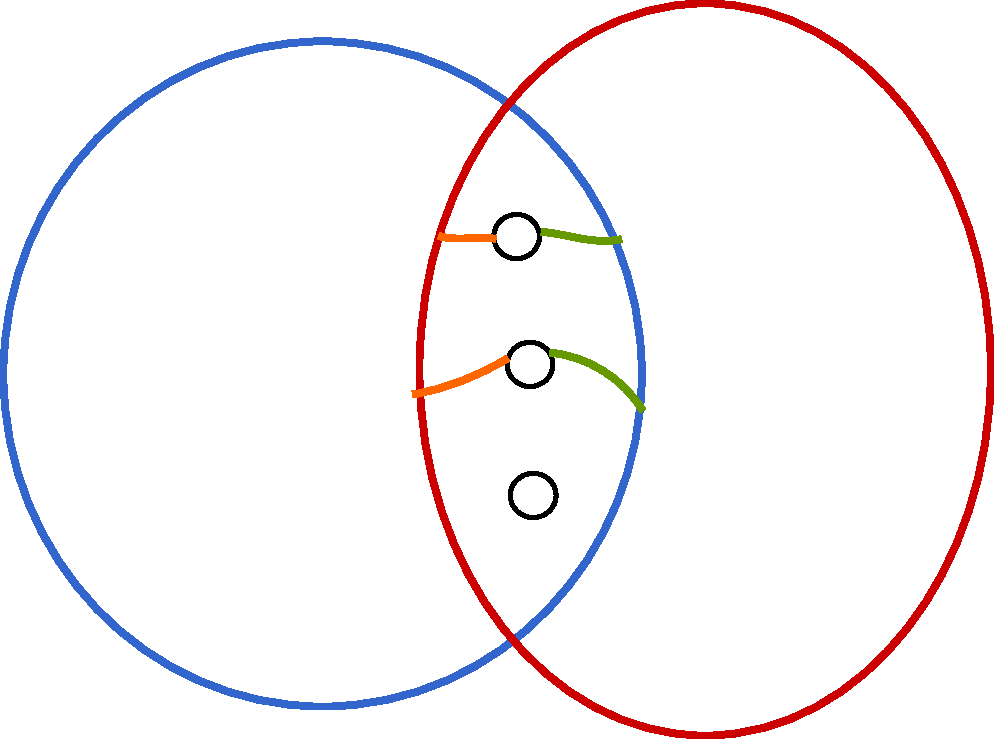
\includegraphics[width=.2\textwidth]{figures/2curveinbigon.pdf}
  No arc of $\alpha,\beta$ can disconnect the band, so the band
  there must contain a path $p_0$ to $p_1$ which is in $y_1$.
  % \includegraphics[width=.5\textwidth]{figures/outofx0.pdf}

\end{proof}


\begin{lemma}
A 3-disk sharing pair uniquely determines a 3-disk.
\end{lemma}
\begin{proof}
  We are working in the 3 \& 4-disk complex of a 5-disk.
  Consider the possible distribution of the marked points
  $p_0,\ldots,p_4$
  in the 5-disk.
  If there is a point that is in none of the 4-disks $y_i$,
  then we would have a hexagon in the 3 \& 4-disk complex of an
  annulus.
  So up to relabeling
  $p_4 \not \in y_0$ and $p_3 \not \in y_1$ and there are
  three cases for 4-disk point configuration

  Case 0: $p_2 \not \in y_2$

  Case 1: $p_4 \not \in y_2$ and $p_2 \not \in x_0$



  Claim that $\partial y_0$ and $\partial y_1$ have
  geometric intersection 2.
  The 3-disk $x_1$ is contained in both $y_0$ and $y_1$.
  So there is only one possible projection for $y_1$ into $y_0$ bands.
  The idea is supposed to be find two arcs in $y_2$
  that you assume are disjoint but the bands get in the way
  Now $p_0,p_3 \in x_0 \subset y_0 \cap y_2$
  and $p_1,p_4 \in x_2 \subset y_1 \cap y_2$.


  Case 2: $p_4 \not \in y_2$ and $p_3 \not \in x_0$

  Claim that $\partial y_0$ and $\partial y_1$ have
  geometric intersection 2.
  The 3-disk $x_1$ is contained in both $y_0$ and $y_1$.
  So there is only one possible projection for $y_1$ into $y_0$ bands,
  which separate $p_3$ from $x_1$ in $y_0$.
  Now  $p_0,p_1,p_2 \in x_2 \subset y_1\cap y_2$ so there must be an arc $\alpha$
  from $p_0$ to $p_1$ contained in $x_2$ but not in $x_1$ so it must
  pass through the bands.
  Similarly $p_0,p_1,p_2 \in x_0 \subset y_2 \cap y_0$
  so there must be an arc $\beta$ from $p_0$ to $p_1$ contained in $x_0$
  but not in $x_1$, so it must cross the bands.
  But then $\beta$ and $\alpha$ form a bigon around $p_3$ so that $p_3$ must be in $x_1$, a contradiction.

  Now $p_0$ and $p_1$
  arc $\alpha$ from $p_0$ to $p_1$
  arc $\beta$ from $p_0$ to $p_1$


  The idea is supposed to be find two arcs in $y_2$
  that you assume are disjoint but the bands get in the way
  Now $p_0,p_3 \in x_0 \subset y_0 \cap y_2$
  and $p_1,p_4 \in x_2 \subset y_1 \cap y_2$.



  Then you're supposed to assume that the $p_0\to p_1$
  arcs in $x_2$ and $x_0$ are not in $x_1$ so they have to be distinct and you force
  them to bound a disk that has to be in $y_2$ and show that defines the 4-curve and
  then its not the one you want?

\end{proof}


\subsection{ Octagonal Sharing Pairs?}

Observe that $C^{ss}(S_1,4)$ is a bipartite graph consisting of
3-disks and 4-disks.

Consider a $2n$-cycle $(x_i,y_i)_{i \in 2n}$ in $C^{ss}(S_{1,4})$
with $x_i$ a 3-disk and $y_i$ a 4-disk.\\

\emph{Claim} Up to relabeling the point configurations of is one of the following three
types:
\begin{enumerate}
  \item $p(x_i) =\{p_i\}_{i \neq j}$
  \item $p(x_0)=p(x_2)=\{p_1,p_2,p_3\}$ and $p(x_1)=p(x_3)=\{p_0,p_1,p_2\}$
  \item $p(x_0)=p(x_1)=\{p_1,p_2,p_3\}$ and $p(x_2)=p(x_3)=\{p_0,p_1,p_2\}$
\end{enumerate}

Fix minimally intersecting representatives of the homotopy classes of octagon
$(x_i, y_i)_{i \in 4}$.\\

\emph{Case 1}\\

If no two 3-disks contain the same 3 points, then up to label permutation
the labels are as above. This configuration is obtained by the following octagon

FIG!!!!


\emph{Case 2}\\

Suppose that  $x_i$ and $x_{i+1}$ contain the same 3 points.
We may assume that $x_0$ and $x_1$ both contain $p_1$, $p_2$, $p_3$.
Consider the image of $x_1$ in $S_{1,4}-x_0$.
Since $x_0$ and $x_1$ are both contained in the 4-disk $y_0$,
there is a unique nontrivial simple closed curve based at the image of $x_0$
in $S_{1,4}/x_0$, so $x_1$ must contain at least one band $b$ so that the
component of $y_0-x_0-b$ containing $p_0$ is a bigon between $b$ and $x_0$.


\includegraphics[width=.5\textwidth]{figures/outofx0.pdf}

The 3-disk $x_2$ has two marked points in common with
$x_0$, suppose without loss of generality that $p_1,p_2 \in x_0 \cap x_2$.
Consider an arc $a_1$ from $p_1$ to $p_2$ in $x_2$.
Assume to the contrary that $a_1$ is not contained in $y_0$.
The 4-disk $y_0$ cannot contain $x_2$.
Then there is an arc $p_2$ to $p_1$ in $x_1 \subset y_0$.
But then $a_1a_2$ is nontrivial curve in the torus,
contained in the 4-disk $y_1 \supset x_1 \cup x_2$, a contradiction.
Then it must be that  $a_1 \subset y_0$.

If $p_0 \notin x_2$, there must be an arc $a_1 \subset x_2$
from $p_1$ to $p_3$ not contained in $y_0$.
Then there is an arc $p_3$ to $p_1$ in $x_1 \subset y_0$.
But then $a_1a_2$ is nontrivial curve in the torus,
contained in the 4-disk $y_1 \supset x_1 \cup x_2$, a contradiction.


We have that $x_2$ contains the points $p_0,p_1,p_2$.
By a similar argument $x_3$ contains the same points.

This configuration is obtained by the following octagon.

FIG!!!!\\

\emph{Case 3}\\

Suppose that $x_{i}$ and $x_{i+2}$ contain the same points.
We may assume that $x_0$ and $x_2$ contain $p_1, p_2, p_3$.
As $x_0$ and $x_2$ are not contained in the same


4-disk there must be two points, say $p_1$ and $p_3$,
and arcs $a_0 \subset x_0$ from $p_1$ to $p_3$
and $a_2 \subset x_2$ from $p_3$ to $p_1$
such that $a_0a_2$ is a nontrivial curve in the unpunctured torus.
Assume to the contrary that $p_1$ and $p_3$ are both in $x_1$,
then there is an arc $a_1 \subset x_1$ from $p_3$ to $p_1$.
Since $a_0a_1 \subset y_1$, we have $a_0a_1$ is nullhomotopic
in the unpunctured torus.
But then $a_0a_2 = rev(a_1)a_2$ is nontrivial in the unpunctured torus
so not contained in $y_2$, a contradiction.
It must be that either $p_1$ or $p_3$ not in $x_1$.
We may assume that $p_3 \notin x_1$.

A similar argument forces $p_1$ or $p_3 \notin x_3$.
Suppose that $p_3 \in x_3$.
Consider an arc $b_3 \subset x_3$ from $p_2$ to $p_3$.
All arcs from $p_1$ to $p_2$ in $x_0$, $x_1$, and $x_2$
must lie in a common 4-curve by the above argument.
But then the arcs from $p_2$ to $p_3$
in $x_0$ and $x_2$ cannot lie in a 4-disk,
but this contradicts that $p_2$ to $p_3$ in $x_3$ lies in both.
It must be that $p_3 \notin x_3$.

This configuration can be realized as follows
FIG!!!!
\qed\\



% \emph{Claim} In an octagon $x_i$ and $x_{i+1}$,
%  there is a unique 2-disk in both $x_i$ and $x_{i+1}$.\\

\emph{Def}
Let $A_{p,q}$
be the set of classes of arcs from point $p$
to point $q$ considered up to homotopy relative to $P$.
By forgetting all the points but $p$ and $q$
we may also consider the arcs $A_{p,q}$
up to homotopy relative to ${p,q}$.
Observe that if $a, a' \in A_{p,q}$
are arcs contained in a common 4-disk then $a$ and $a'$ are homotopic relative to $\{p,q\}$.

\vspace{1cm}

\emph{Claim} Suppose that $x_0$ and $x_2$ are distance four
3-disks in an octagon.
Then $x_0$ and $x_2$ contain the same points
if and only if there more than 2 length 4 paths from $x_0$ to $x_2$.\\
\\
Suppose that there are at least 3 paths from $x_0$ to $x_2$,
each of which pass through a distinct 3-disk, say $x_1$, $x_2$, $x_3$.
If $x_1$, $x_2$, $x_3$ all contain distinct sets of marked points,
then by the possible point configurations
described by Lemma !!!!, there are not possible choice for the
marked points contained in $x_0$ and $x_2$.
If two of  $x_1$, $x_2$, $x_3$ contain the same points.
But then by the possible point configurations
described by Lemma !!!!, the $x_0$ and $x_2$ must also contain the same points.

Suppose $x_0$ and $x_2$ contain the same points, say $p_1,p_2,p_3$.
Then by the Lemma !!!!
it must be that $x_1$ and $x_3$ contain the same points,
say $p_0,p_1,p_2$.
Suppose that there is a nonseparating curve $\alpha$ based at $p_0$
and disjoint from $x_0$ and $x_2$.
Let $$x_0,y,x,y',x_2$$ be a length 4 path.
Since $p_0 \in y,x,y'$
we have that
$$x_0 \to T^k_\alpha y \to T^k_\alpha x \to T^k_\alpha y'\to x_2$$
gives infinitely many paths of length 4.

If there is no nonseparating curve then $p_0$ is in 2n-gon. Connect p0 to all the corners!





 \emph{Claim}
 Up to homeomorphism
 there is only one
 type of octagon with $p(x_i) =\{p_j\}_{j \neq i}$.\\
 \\



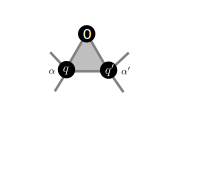
\includegraphics[width=.5\textwidth]{figures/nobigonsrotycase.pdf}

Consider the two 3-disks
$x_0$ and $x_2$. Observe that $x_0$ and $x_2$ cannot be contained in
a common 4-disk, or else $x_0,x_1,x_2$ would all be contained in a common
4-disk which would force $y_0=y_1$ by Lemma !!!!.

Assume to the contrary that $x_0$ and $x_2$
contain a common arc $a_{13} \in A_{p_1,p_3}$.
Consider arcs $a^{(0)}_{12} \in A_{p_1,p_2}$ in $x_0$
and $a^{(2)}_{10} \in A_{p_1,p_0}$ in $x_2$
which cannot be contained in a common 4-disk,
since otherwise a regular neighborhood of $a_{12} \cup a^{(0)}_{13} \cup a^{(2)}_{01}$
is a 4-disk containing $x_0$ and $x_2$.
Then $x_3$ contains arcs
$a^{(3)}_{12} \in A_{p_1,p_2}$,
which must be homotopic to $a^{(0)}_{12}$ relative to $p_1,p_2$,
and
$a^{(3)}_{10} \in A_{p_1,p_0}$,
which must be homotopic to $a^{(2)}_{10}$ relative to $p_1,p_0$.
But then $a^{(3)}_{12}$ and $a^{(3)}_{10}$
cannot be contained in a common 4-disk, and yet are contained in $x_3$, a contradiction.

Let $a^{(i)}_{i+1,i+2} \in A_{p_{i+1}, p_{i+2}}$ for $i \in 4$
be an arc in $x_{i}$.
Then we have a
loop $a=a^{(0)}_{12}a^{(1)}_{23}a^{(2)}_{30}a^{(3)}_{01}$
of $S_1$.
We may assume any self-intersections of $a$ occur
transversely at points not in $P$.

Assume to the contrary that $a$ is nullhomotopic in $S_1$.
% Then there is a non-embedded disk $D\subset S_1$
% with $\partial D = a$ which cannot be contained in a 4-disk of $S_{1,4}$.
So $a$ must be a non-simple separating curve in the torus.
There must be a point $p \in P$
such that $a$ is not nullhomotopic relative to $\{p\}$.
Relabel $P$ so that $a$ is not nullhomotopic relative to $\{p_0\}$.
So $a$ forms an innermost bigon $b$ with itself with $p_0$ on one side.
Let $q,q' \in a$ be the vertices of the bigon.
\includegraphics[width=.5\textwidth]{figures/abigon.pdf}
The image of $a-(b-q)$ must contain a simple closed curve $\alpha$ based
at $q$,
and
$a-(b-q')$ contains a simple closed curve $\alpha'$ based
at $q'$.
Since $a^{(i)}$ and $a^{(i+1)}$ must be contained in a common 4-disk,
their union cannot contain loops of the torus.
So both $\alpha$ and $\alpha'\subset a$
must have at least 2 points of $P -\{0\}$, but
they do not intersect at $P$, a contradiction.

Assume to the contrary that $a$ is not homotopic in $S_1$
to a simple closed curve of $S_1$.
Let $q$ be a self-intersection of $a$
and let $\alpha$ and $\alpha' \subset a$ be two nontrivial loops of $S_1$
sharing no common subarcs.
Then $\alpha$ and $\alpha'$ must each contain two points of $P$.
Say $\alpha$ contains $p_0$ and $p_1$ while $\alpha'$ contains $p_2$ and $p_3$.
So $a^{(0)}_{12}$ and $a^{(2)}_{30}$
must intersect at $q$.
Observe $x_1$ must contain an arc $a^{(1)}_{30} \in A_{p_3p_0}$
homotopic to $a^{(2)}_{30}$ relative $\{p_3p_0\}$
and disjoint from $a^{(1)}_{23} - \{p_3\}$.
Then $a^{(2)}_{30}$ and $a^{(1)}_{30}$ cannot be homotopic relative to $P$,
as if $a^{(1)}_{30}$ intersects $a^{(0)}_{12}$
the 4-disk $y_0$ would contain $\alpha'$.
Then $a^{(1)}_{23}$ must
link with $a^{(3)}_{01}$.
But then $a^{(3)}_{01}$ is homotopic relative $\{p_0,p_1\}$
to a curve
$a^{(2)}_{01} \in A_{p_0p_1}$ in $x_2$ which must link with $a^{(1)}_{23}$.
But then $y_1 \supset x_1\cup x_2$ contains a nontrivial loop of the torus.
It must be that $a$ is a homotopic in $S_1$ relative
$\varnothing$ to a simple closed curve of $S_1$.

Let $b$ be the simple closed curve obtained from $a$
by homotoping the arcs $a^{(i-1)}_{i,i+1}$ relative ${p_i,p_{i+1}}$.
We may assume that $a^{(3)}_{01}=b^{(3)}_{01}$.
\includegraphics[width=.5\textwidth]{figures/stayinannulus.pdf}
Assume to the contrary that
$a^(0)_{12}$
is not supported on the annulus $N(b)$.
Then let $D$ be an innermost bigon formed by $a^{(0)}_{12}$ and
$b^{(3)}_{12}$, which must contain
a point of $P-\{p_1,p_2\}$.

If
$a^{(0)}_{12}$ and
$a^{(3)}_{01}$ intersect at a point $q \in \partial D$,
then $a^{(3)}_{01}$ has an arc that cros
 $a^{(0)}_{12}$
contains a loop

% Since $p_1,p_2 \in D$ it must be that
% $a^{(3)}_{01}$ intersects
% $b^{(0)}_{12}$ an even number of times, including $p_1$,
% so the interior of the arcs intersect an odd number of times.
% So the interiors of $a^{(3)}_{01}$ and $a^{(0)}_{12}$
% intersect an odd number of times. Let $q$ be such an intersection point.
% Then $a^{(3)}_{01} \cup a^{(0)}_{12}$ contains an arc $b'_{12}$ which cannot



% Assume to the contrary that $x_0$ and $x_3$ do not contain a common
% 2-disk.
% Let $z \subset x_0$ be a 2-disk containing $p_1$ and $p_2$
% Consider the image of $x_3$ in $S_{1,4}/z$.
% As  $p_0 \in x_3$ the 3-disk $x_3$ must contain a bigon containing $p_0$
% with one edge on $\partial z$.
% It must be that $x_3$ contains a band $b \subset y_3$
%  winding around $p_0$ to connect $p_1$ and $p_2$.
% Further $x_3$ must contain a band $b' \subset y_3$ winding around $p_3$ to connect
% $p_0$ to $p_1,p_2$.
% As $x_3 \not \subset y_1$ there must be a nonseparating curve $\alpha \subset y_1^c$
% that intersects $x_3$. Since $\alpha$ is disjoint from $x_0$,
% it must separate $y_3$ into components containing $p_0$
% and separately $p_1,p_2,p_3$.
% This forces the components of $x_3 - \alpha$ to separate $p_1$  from
% $p_2$
% from $p_3$.
% Then there is an arc $a_1 \subset x_1$ from $p_0$ to $p_3$.
% Since $a_1$ is disjoint from $\alpha$ it has a nontrivial image in $S_{1,4}/y_3$.
% Consider an arc $a_2 \subset x_2$ from $p_3$ to $p_0$.
% Since $a_1a_2 \subset y_1$ is trivial in the unpunctured torus,
% $a_2 \not \subset y_3$ and $a_2$ must have
% parallel arcs to $a_1$ in $S_{1,4} -y_3$.
% If $a_2$ is disjoint from $\alpha$, then $x_3 \cup a_2$
% contains a nontrivial loop in the unpunctured torus, contradicting that $x_3\cup a_2 \subset y_2$.
% So $a_2$ must intersect $\alpha$.
% Consider the subarc $a_1' \subset a_1 \cap y_3$
% from a point $q_0 \in \partial y_3$ to $p_0$.
% Since $a_2$ intersects $\alpha$ it must intersect $a'_1$.
% But then $a_1 \cup a_2$ cannot be contained in $y_1$, a contradiction.
% It must be that $x_0$ and $x_3$ contain a common 2-disk.\\


%  \emph{CASE 2}
%  Suppose
% $p(x_0)=p(x_2)=\{p_1,p_2,p_3\}$ and $p(x_1)=p(x_3)=\{p_0,p_1,p_2\}$
%  \\
%
% Observe all curves contain the points $p_1$ and $p_2$.
% Assume to the contrary that $x_0$ and $x_3$ do not contain a
%
%
% COLLAPSE 3-disks to look throw out arcs that aren't contained in adjacent 3-disks.
% %
% Consider the image of $x_3$ in $S_{1,4}-x_0$.
% The 3-disks $x_0$ and $x_3$ must be contained a 4-disk $y_3$ distinct from $y_1$,
% so $x_3$ contains either a similar band $b'$ such that $b'^c \cap b^c$ contains a bigon containing $p_0$,
% or $x_3$ contains a bigon containing $p_0$ with one side on $x_0$.
% Consider the 4-disk $y_2$, which contains $x_2$ and $x_3$.
% If $y_2$ also contained $x_0$, then $y_2$ would be a 4-disk containing $x_3$ and $x_0$,
% and we would have $y_2$ homotopic to $y_3$, a contradiction.
% So $y_2$ must  intersect $x_0$, and in particular
% we must be able to write $y_2$ as the complement of a regular neighborhood of
% a pair of intersection 1 nonseparating arcs $\alpha$ and $\beta$
% with $\alpha$ intersecting $x_0$.
% % Observe that $\alpha$ is disjoint from $x_2$ and $x_3$
% So $\alpha$ cuts  $y_0$ into at least two components.
% Since $x_3$ and $x_0$ contain at least two points in common
% we may assume $p_1$ and $p_2$ are contained in $x_0$ and $x_3$.
% Then as $\alpha$ intersects $x_0$ but not $x_2 $in $y_3$, it must be that
% $p_1$ and $p_2$ are contained in a common component of $x_0 -\alpha$
% and a different component than $p_3$.
%
%
%
%
% Consider what points $x_2$ may contain.
% Suppose that $p_3 \in x_2$.
% As $x_2$ must contain $p_1$ or $p_2$,
% say $p_1 \in x_2$.
% Then $x_2$ contains an arc $a_2$ from $p_1$ to $p_3$
% Observe that $a_2\subset x_2 \subset y_2$ is disjoint from $\alpha$.
% So $S_1 -\alpha$ is an annulus with
%
% But $x_1$ contains an arc $a_1$ from $p_3$ to $p_1$
% which must intersect $\alpha$
% an odd number of times as $p_3$ and $p_1$
%  are in separate components of $y_0-\alpha$.
% So $a_1a_2$ gives a nontrivial nonseparating curve in the torus and
% contained in $y_1$, contradicting that $y_1$ is a 4-disk.
%
% Then $p_0,p_1,p_2 \in x_2$, so the band $b$ intersects $x_2$ since $x_2$ is not contained in $y_1$.
% But then $x_2$ and $x_1$ cannot be contained in a common 4-disk.\qed






\noindent \emph{Remark }
Fix a 2-disk $z$
A pair ${x,x'}$ of 3-disks containing $z$ are
a sharing pair for $z$ if they fit into a common octogon.
Call a triple ${x,x',x''}$ of 3-disks containing $z$
a sharing triple if every two form a sharing pair.

Make a graph $P_z$ whose vertices are sharing pairs ${x,x'}$
of $z$ and with two sharing pairs adjacent if
their union is a sharing triple.

Well-definedness is shown by Putman's Lemma on $P_z$.
Observe that only two of the generators move the sharing pair
at all and only distance 1.

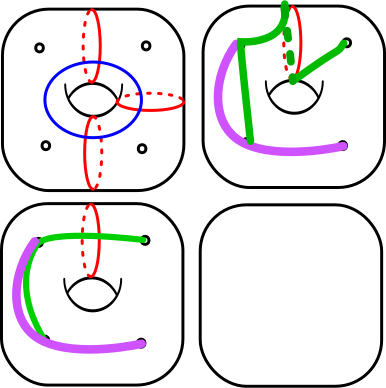
\includegraphics[width=.5\textwidth]{figures/s14.pdf}


\section{Computational Evidence}

Fix a triangulation of the surface with all points at the marked points.

Data is a triangulation $T$
\begin{enumerate}
  \item A triangulated polygon embedded in the plane $\R^2$
  \item List of oriented triangles given by triples of directed edges
\end{enumerate}

Normal coordinates
Laminations are functions $f: T \to \R$
Multicurves are integer laminations $f: T \to \Z_{\geq 0}$


$S_{1,4}$ has triangulation
 $$
 \begin{tikzcd}
   p_0 \arrow{r}{e_0} & p_1 \arrow{r}{e_3} & p_2 \arrow{r}{e_6} & p_3 \arrow{r}{e_9} & p_0\\
   p_0 \arrow{r}{e_0} \arrow{u}{e_1} & p_1 \arrow{ul}{e_2} \arrow{r}{e_3} \arrow{u}{e_4} & p_2 \arrow{ul}{e_5} \arrow{r}{e_6} \arrow{u}{e_7} & p_3 \arrow{ul}{e_8} \arrow{r}{e_9}  \arrow{u}{e_{10}} & p_0 \arrow{ul}{e_{11}} \arrow{u}{e_1}
 \end{tikzcd}
 $$

Normal coordinates
uniquely
determine a number of line segements at each angle of each triangle

Also write as crossing sequence, cyclic reduced word in $T^{\pm}$

Computing dehn twists

possible in polynomial time

simplify  $T_\alpha(\beta)$ computation by a choice
of end for every edge so that $\alpha$ always passes through the end
and $\beta$ always passes through the middle

Hyperbolicity constant of the curve graph
Hyperbolicity constant of the strongly separating curve complex

Github

%---------------------------%
%###########################%
%---------------------------%
\section{Complex of Surfaces}

\noindent \emph{Def}
A genus $g$ \emph{rosebud} is the wedge of a sphere and a genus $g$ rose.
We consider spheres genus 0 rosebuds, and roses degenerate rosebuds.\\
\\

\noindent \emph{Claim}
Every embedded compact
closed orientable surface in $M_g$
is homotopy equivalent to a sphere, rose, or rosebud.\\
\\
\emph{Proof.}
Consider the image in $S^3$ minus spheres.
Every disk is compressible.\qed\\
\\

\noindent \emph{Claim}
An embedded surface $S_g$ has $\pi_1(S_g)$ contains a
free factor at most rank $g$.\\
\\
\emph{Proof.}
If $\pi_1(S \hookrightarrow M)$ contains a free factor rank $k$,
then $S$ intersects at least $k$ disjoint spheres
in $M$. Then there are at least $k$
compressible disks with $\partial D \subset S$.
Each one kills a generator of $\pi_1(S)$
\\

\noindent \emph{Claim}
There is a correspondence between
homotopy classes of embedded rosebuds
in $M_n$ and one edge Bass Serre graph-of-groups
decompositions of $F_n$.\\
\\
\emph{Proof.}
By Van Kampen every rosebud gives a graph of groups.
Conversely if $F_n =  \pi_1 ( A \leftrightarrow C \rightarrow B )$
then there is a basis $\{a_i\}_{i \in n}$ of $F_n$
with the first $k$ in $A$ and the last $n-k$ in B.
This corresponds to a system of nonseparating spheres.
There is a unique separating sphere $S$ which separates the $A$
spheres from the $B$ spheres.
From a basepoint on $S$ there is a rose whose petals give the arcs forming
a basis of $C$. \qed\\
\\

\noindent \emph{Def. }
The graph of embedded rosebuds
$\mathcal R_n$
has embeddings of rosebuds (and roses) of genus at most $n$ as vertices.
Two embedded rosebuds are adjacent if the embeddings of their
homotopy classes differ by
the wedge of a (homologically nontrivial?) 1- or 2-sphere.\\


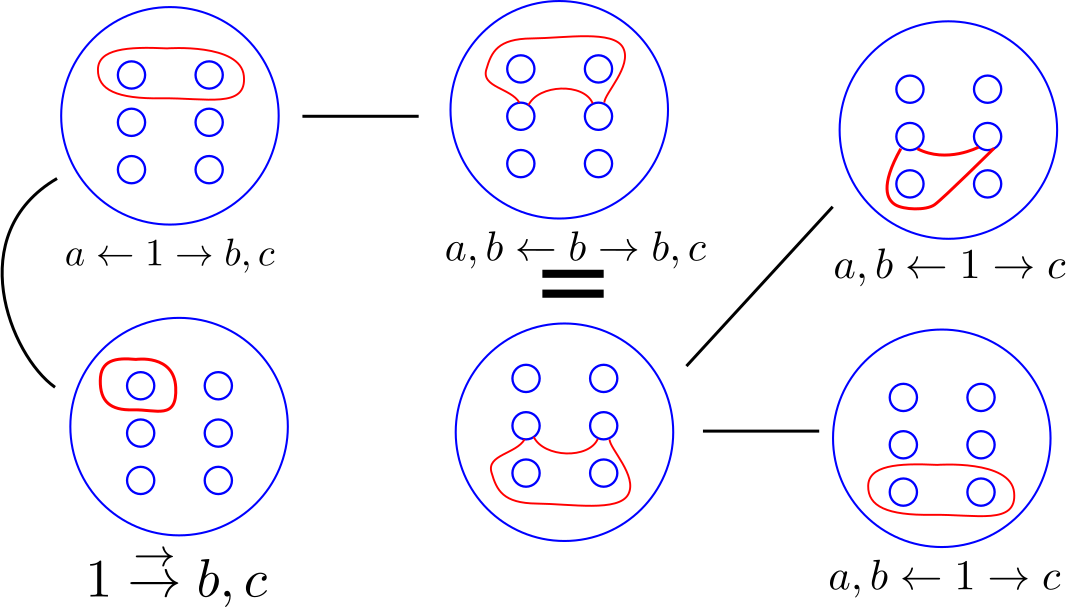
\includegraphics[width=.8\textwidth]{figures/rosebudgraph.pdf}


$\mathcal R_n$ is equivalent to the graph of one-edge Bass Serre
graph-of-group decompositions of $F_n$ with adjacency given by
the following moves:
\begin{enumerate}
  \item tube tunneling at $a \in A - B$
  $$A \leftarrow C \rightarrow B  \ \Leftrightarrow  \ A \leftarrow C \ast a \rightarrow B \ast a$$
  \item nonseparating sphere scooping (primitive $b \not \in A$)
  $$
   C \stackrel{\rightarrow}{\rightarrow} A \ast A'b
    \ \Leftrightarrow  \
    C \stackrel{\rightarrow}{\rightarrow}  A \ast A'
     \ \Leftrightarrow  \
  b \ast C \leftarrow C \rightarrow  A \ast A'
  $$
\end{enumerate}

%%#-------------------------------



\nocite{*}

\bibliography{references}{}
\bibliographystyle{plain}
\end{document}
